\documentclass[12pt]{article}
\usepackage{geometry}
\geometry{a4paper, margin = 1in, left = 1.2in}
\usepackage{graphicx}
\graphicspath{{D:/Reef/Work/GitHub/Project_2/Image/}}
\usepackage{float}
\usepackage{csvsimple}
\usepackage{pgfplotstable}
\usepackage{booktabs}
\usepackage{caption}
\usepackage{subcaption}
\usepackage{fancyvrb}
\usepackage{xcolor}
\usepackage[utf8]{inputenc}
\PassOptionsToPackage{hyphens}{url}
\usepackage[hidelinks]{hyperref}
\usepackage{listings}

\begin{document}
\begin{titlepage}
	\begin{center}
		
		{\bfseries DIY Automatic Delivery Trolley} \\
		[1cm]
		by \\
		[1cm]
		Utchawin Namdee\\ 
		\medskip
		Patipan Arunwattanawong \\
		[1cm]
		A report submitted in partial fulfillment of the requirements for \\
		the degree of Bachelor of Engineering in \\
		Mechatronics Engineering \\
		[1cm]
		Project Advisor:\\
		\medskip
		Asst. Prof. Dr. Narong Aphiratsakun \\
		[1cm]
		Examination Committee: \\
		[1cm]
		Dr. Jerapong Rojanarowan, Dr. Wisuwat Plodpradista, \\
		Assoc. Prof. Dr. Jiradech Kongthon, Mr. Sunchanan Charanyananda, \\
		Mr. Amulya Bhattarai, Mr. Ehsan Ali \\
		[1cm]
		Assumption University \\
		Vincent Mary School of Engineering\\
		Thailand \\
		October 2020 \\
		
	\end{center}
\end{titlepage}

\newpage
\thispagestyle{empty}

\noindent Approved by Project Advisor:\newline
\hspace*{7cm} Name: Asst.Prof.Dr. Narong Aphiratsakun \\
\hspace*{7cm} Signature:\\
\hspace*{7cm} Date:\hrulefill \\
[1cm]
Plagiarism verified by: \\
\hspace*{7cm} Name: Mr. Ehsan Ali \\
\hspace*{7cm} Signature: \\
\hspace*{7cm} Date:\hrulefill \\

\newpage
\pagenumbering{roman}
\addcontentsline{toc}{section}{\numberline{}Abstract}

\section*{Abstract}\label{sec:abs}

\indent This project will describe the automatic delivery trolley for sending documents to a specific station. This system is able to deliver documents without human interaction using trolley mechanisms. Various type of documents can be sent/receive to and from several stations. Moreover, the trolley system can be control using command issue via mobile application. The system consists of infrared (IR) sensor to make the trolley run along the black line and ultrasonic sensor to avoid colliding with objects or people. This project can be used in various physical/environmental situations. For example, sending the documents or medicine in the hospital, homes with elderly or disabled people. In addition, the scale can be developed or expanded to use other works like transporting various parts in the factory or transportation between cities.

\newpage

\tableofcontents
\thispagestyle{empty}

\newpage
\pagenumbering{arabic}

\setcounter{page}{1}

\section{Introduction} \label{sec:intro}

\subsection{Introduction of Topic} \label{subsec:intro}

Nowadays, automation industrial plays significant role in the world as we can see in the daily life such as automatic door and vacuum cleaner robot. We can say that automation technology initiates other technology so that they have their own names and branch, for example, Robotics. We as a student would like to apply some automation technology to a daily life so that others can easily access to it. What we are going to do is DIY automatic delivery trolley.

\subsection{Project Objective} \label{subsec:project obj}

Delivery something to someone might be a hard time if there is far distant between them. So, we develop this DIY automatic delivery trolley to solve this problem. The user will use smart phone application to control the Trolley to deliver the item from one place to another.

\section{Project Overview} \label{sec:project over}

\subsection{Initial study \& Background study} \label{subsec:initial study}

Currently, there are many types of controller, but we found 2 main types of controller that are suitable for our project: Arduino and Raspberry Pi. \par
Raspberry Pi resembles a mini PC but use an OS that is developed from Linux. For the Raspberry Pi can use Python C++ to write the command. \par
Arduino is a microcontroller which can only work in accordance with the program that we wrote and there is no built-in OS. It is designed to be economical, small, does not require additional equipment for uploading sketches. there is also a port to connect with external sensors more than Raspberry Pi. There are various protocols which is a standard for connecting with external hardware for example I2C, SIP, UART including both Digital and Analog port. Importantly, it works more specifically type than Raspberry Pi for example real time control Arduino is more suitable than Raspberry Pi. In addition, Arduino is also designed the system to prevent over-voltage better than Raspberry Pi.

\section{System} \label{sec:system}

\subsection{Block diagram of the System} \label{subsec:block diagram}

\begin{figure}[H]
	\centering
	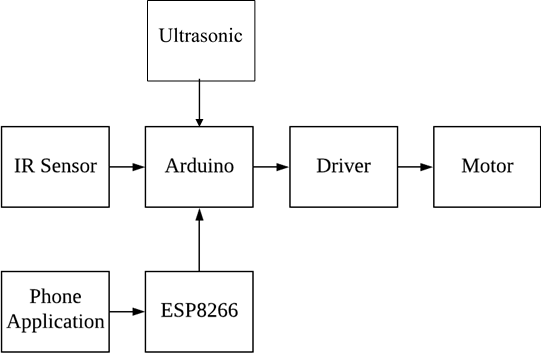
\includegraphics[height= 6cm]{Blockdiagram}
	\vspace{0.1cm}
	\caption{Block diagram of the system} \label{fig:block}	
\end{figure}

The block diagram shown in Figure \ref{fig:block} depicts how our system works. Firstly, the microcontroller, Arduino, will receive the data from sensors and ESP8266. Then Arduino will send it to driver. Lastly, the driver will drive the motor.

\subsection{Controller} \label{sub:controller}

\subsubsection{Arduino Uno Board} \label{subsub:arduino}

\begin{figure}[H]
	\centering
	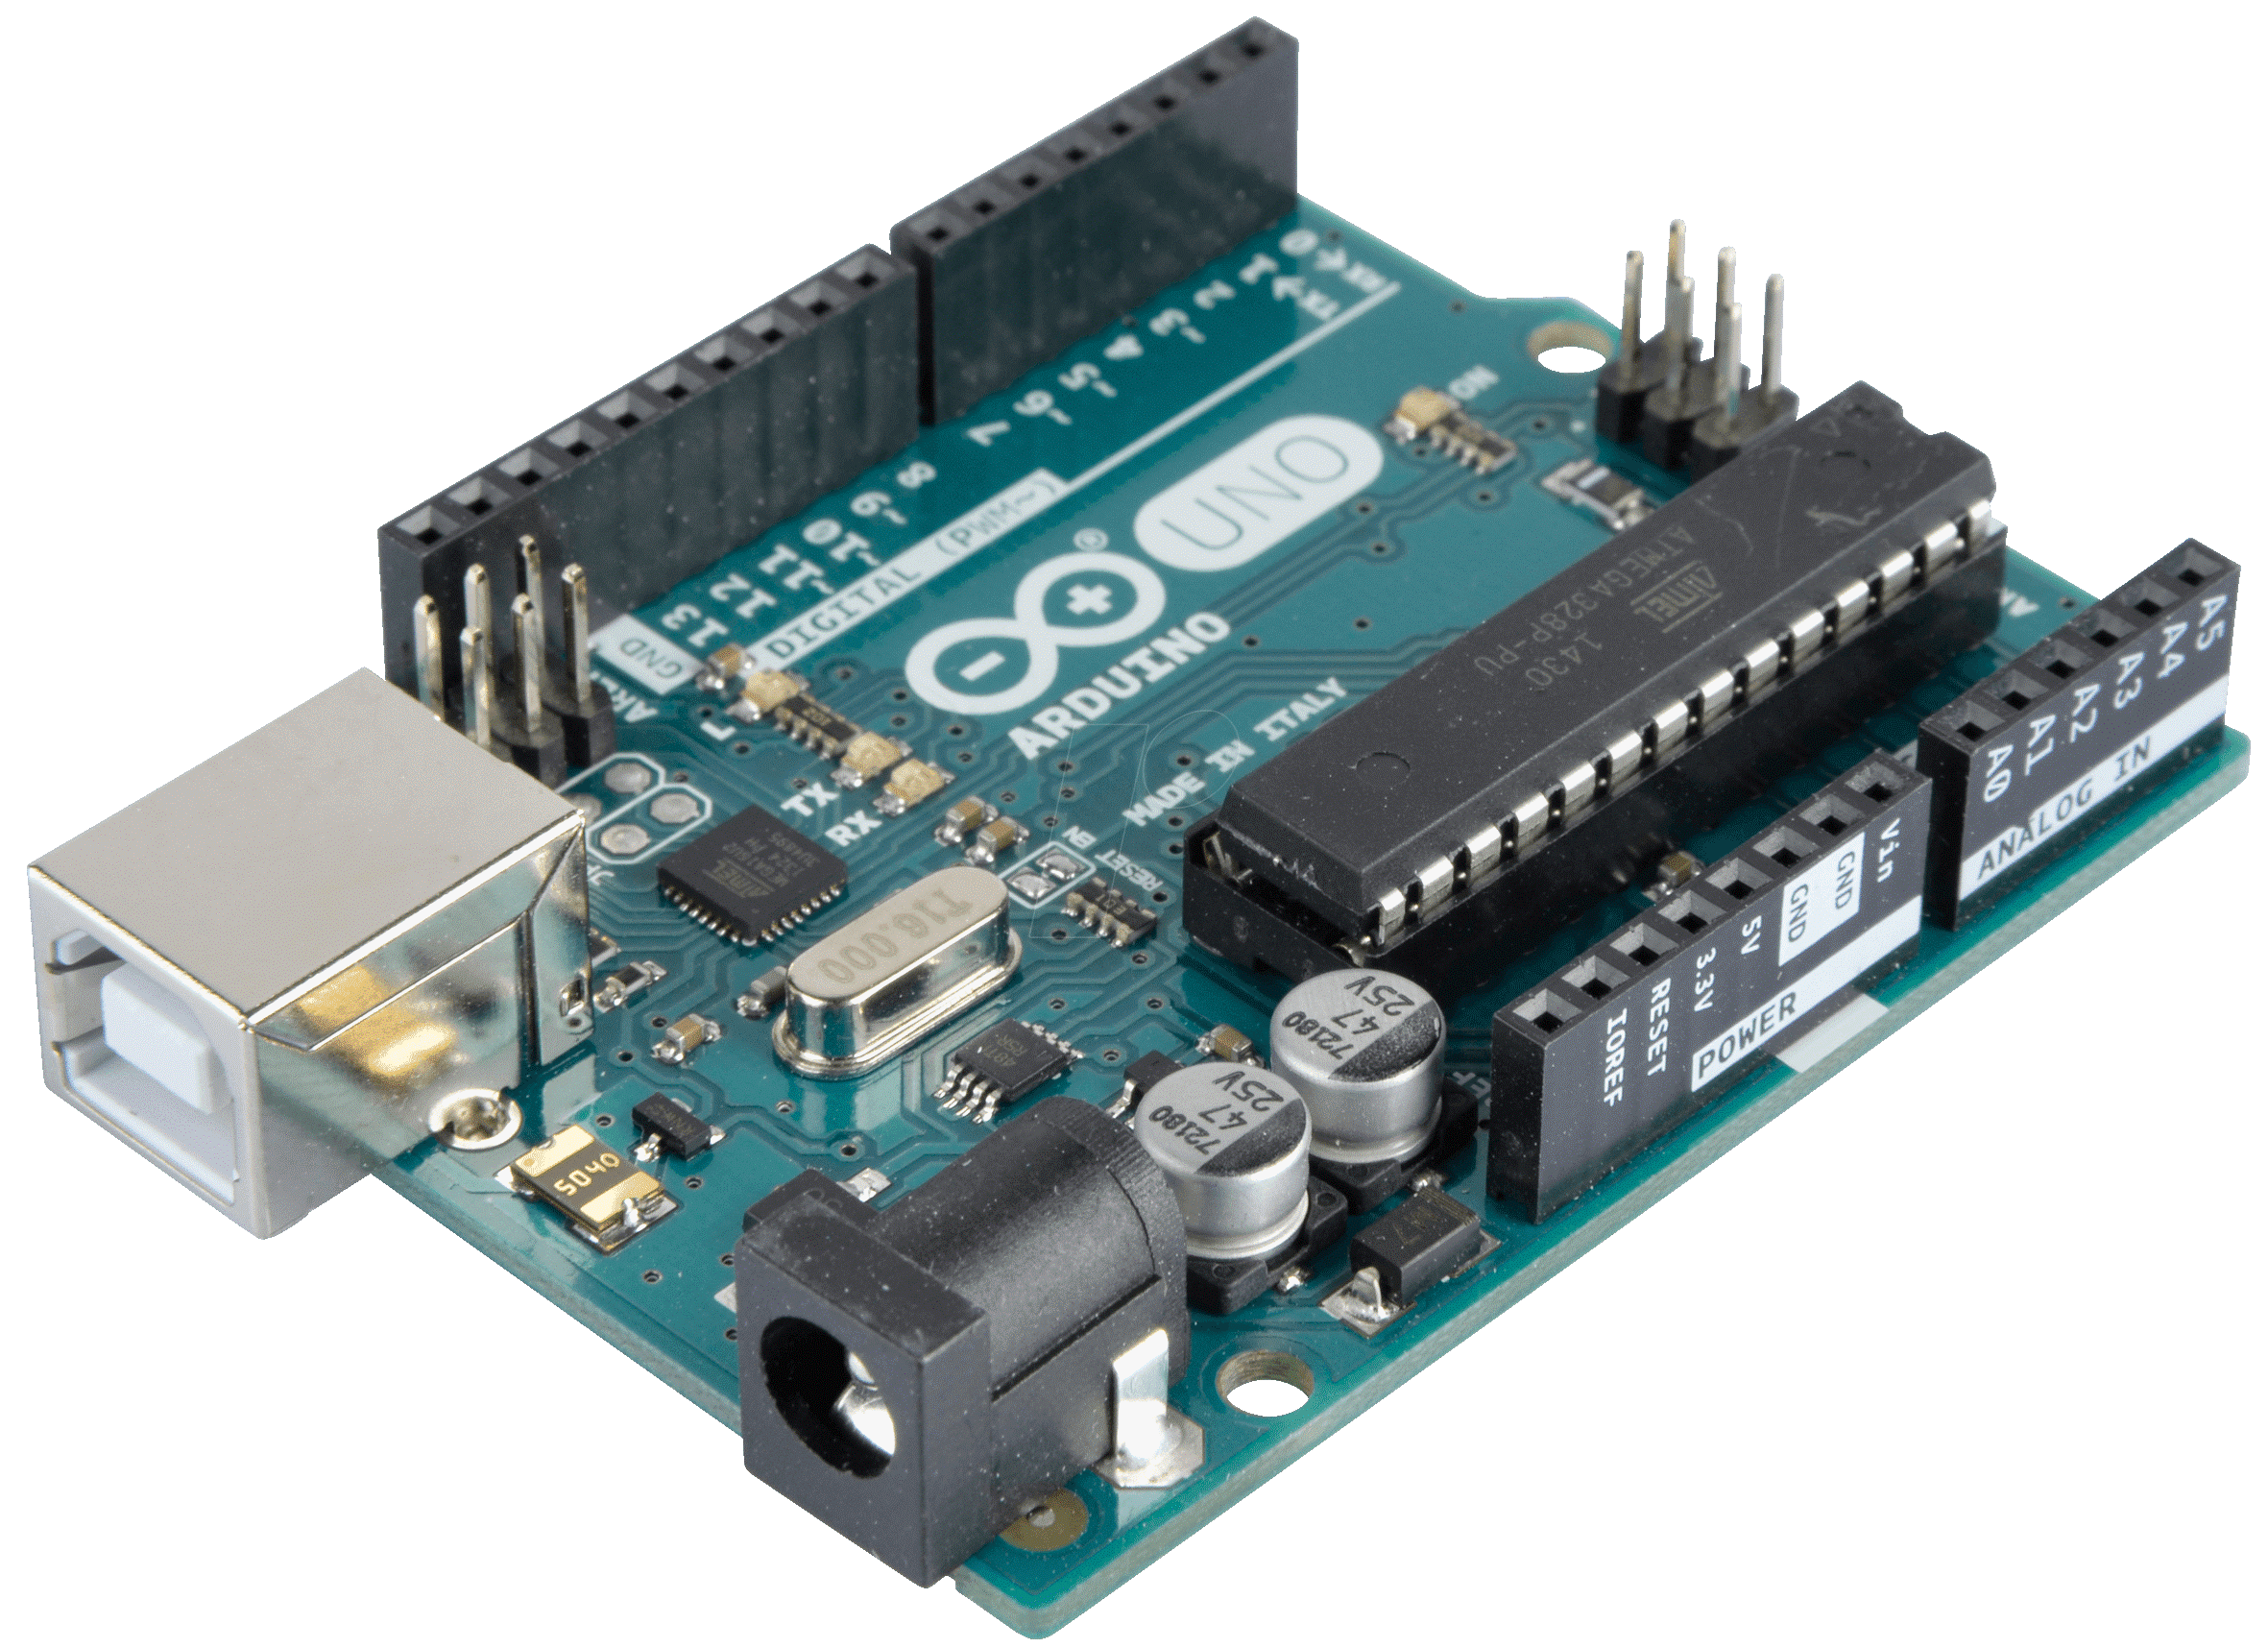
\includegraphics[height= 5cm]{ArduinoUno}
	\caption{Arduino UNO Board} \label{fig:arduino}
\end{figure}

The Microcontroller that we are going to use is Arduino UNO since it is a beginner friendly and easily to code. Arduino UNO, operating at 5V, comes with 14 Digital input and 6 Analog input which is more than enough for this project. Using Arduino UNO make us applied what we have learned so far in the classroom into the real world. Furthermore, Arduino UNO are used in various of projects around the world so that we can have many references and support as we want. We use Arduino UNO to be the main controller.

\begin{table}[H]
	\centering
	\label{tab:arduino}
	\caption{Specification of Arduino UNO}
	\pgfplotstabletypeset[
	col sep=comma,
	string type,
	every head row/.style = {before row=\toprule ,after row = \midrule},
	every last row/.style ={after row = \bottomrule},
	columns/No./.style={column type = l}]{Arduino.csv}
\end{table}

\subsubsection{ESP8266} \label{subsub:esp}

\begin{figure}[H]
	\centering
	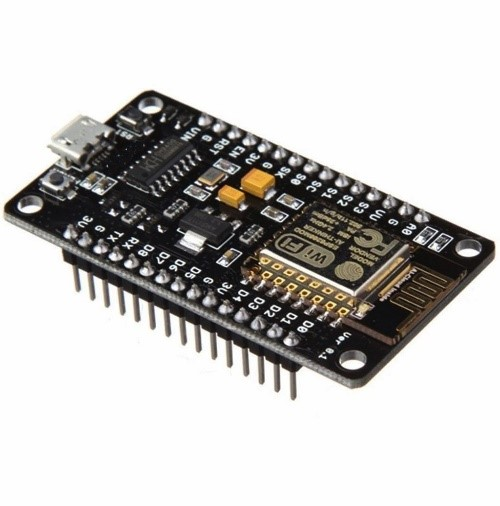
\includegraphics[height= 5cm]{ESP8266}
	\caption{ESP8266 Board} \label{fig:esp}
\end{figure}

\normalfont The ESP8266 is another microcontroller that we use in this project. This MCU has a Wi-Fi receiver so that we can communicate it via application in the smart phone. The communication will start from the application to ESP8266 via WiFi and then back to Arduino UNO via serial communication. We use this controller to connect the application to Arduino for entering commands via the application.

\begin{table}[H]
	\centering
	\label{tab:esp}
	\caption{Specification of ESP8266 Board}
	\pgfplotstabletypeset[
	col sep=comma,
	string type,
	every head row/.style = {before row=\toprule ,after row = \midrule},
	every last row/.style ={after row = \bottomrule},
	columns/No./.style={column type = l}]{ESP8266.csv}
\end{table}

\subsection{Sensors} \label{sub:sensors}

\subsubsection{Infrared (IR) Obstacle Avoidance Sensor Module} \label{subsub:ir}

\begin{figure}[H]
	\centering
	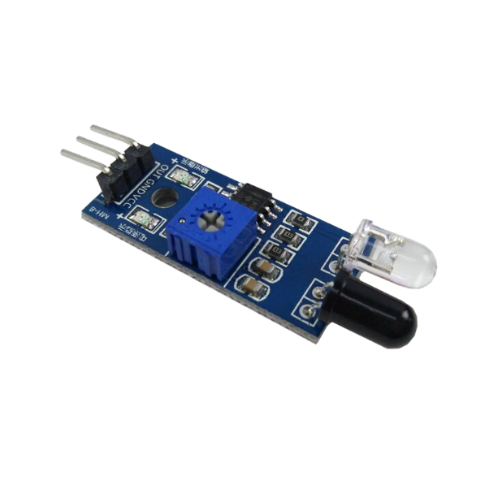
\includegraphics[height= 5cm]{Infrared}
	\caption{Infrared (IR) Sensor} \label{fig:ir}
\end{figure}

IR Infrared Obstacle Avoidance Sensor Module, working under voltage of 3.3 to 5 V DC, is an optical sensor for detecting obstructions or black surfaces. Receiver will always be able to receive the light signal from Emitter transmitter if the surface is not black and the value is 0. On the other hand, emitter sent the signal to the black surface Therefore, the Receiver cannot receive the signal from reflection then the value is 1. From this project we use them to detect black line in order to make the trolley run along the black line. We use IR infrared to detect the black line is defined.

\subsubsection{Ultrasonic Sensor HC-SR04} \label{subsub:ultra}

\begin{figure}[H]
	\centering
	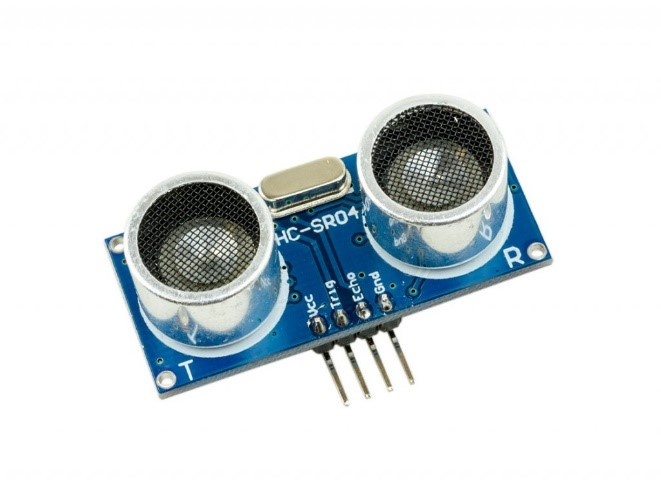
\includegraphics[height= 5cm]{Ultrasonic}
	\caption{Ultrasonic Sensor HC-SR04} \label{fig:ultra}
\end{figure}

Ultrasonic Sensor HC-SR04 is used for detecting obstacles in front to prevent accidents. We use ultrasonic to prevent collisions with objects or living things.

\begin{table}[H]
	\centering
	\label{tab:ultra}
	\caption{Specification of ESP8266 Board}
	\pgfplotstabletypeset[
	col sep=comma,
	string type,
	every head row/.style = {before row=\toprule ,after row = \midrule},
	every last row/.style ={after row = \bottomrule},
	columns/No./.style={column type = l}]{Ultrasonic.csv}
\end{table}

\newpage 

\subsection{Driver and Motor} \label{sub:drivernmotor}

\subsubsection{Motor Driver Module L298N} \label{subsub:driver}

\begin{figure}[H]
	\centering
	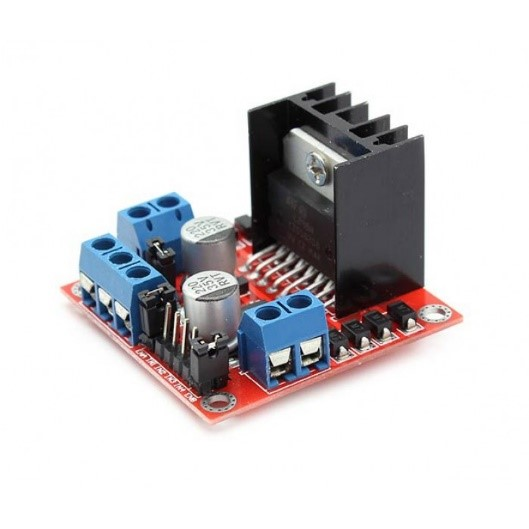
\includegraphics[height= 5cm]{Driver}
	\caption{Motor Driver Module L298N} \label{fig:driver}
\end{figure}

Motor Driver Module L298N is used for motor driving, speed control and direction control. We will use the module to control speed and direction along the black line. The operating voltage is 7 to 35 V DC and the maximum current that this driver can handle is 2 A.

\subsubsection{Motor} \label{subsub:motor}

\begin{figure}[H]
	\centering
	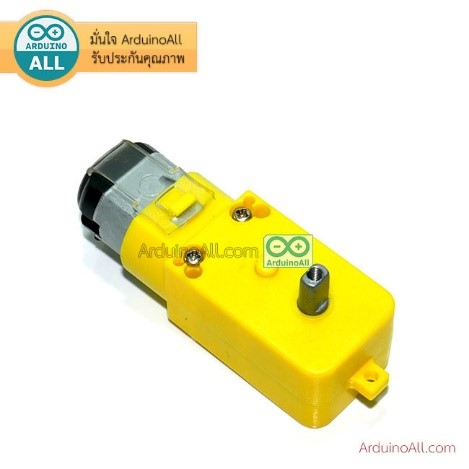
\includegraphics[height= 5cm]{Motor}
	\caption{Motor} \label{fig:motor}
\end{figure}

Motors are used for running the trolley. For this project we decide to use 2 motors to run the trolley.

\begin{table}[H]
	\centering
	\label{tab:motor}
	\caption{Specification of Motor}
	\pgfplotstabletypeset[
	col sep=comma,
	string type,
	every head row/.style = {before row=\toprule ,after row = \midrule},
	every last row/.style ={after row = \bottomrule},
	columns/No./.style={column type = l}]{Motor.csv}
\end{table}

\subsection{Miscellaneous} \label{sub:misc}

\subsubsection{Metal Bars with screw holds} \label{subsub:metal}

\begin{figure}[H]
	\centering
	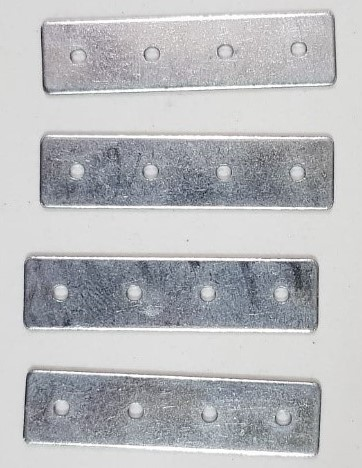
\includegraphics[height= 5cm]{Metal}
	\caption{Metal Bars} \label{fig:metal}
\end{figure}

\subsubsection{Switch} \label{subsub:switch}

\begin{figure}[H]
	\centering
	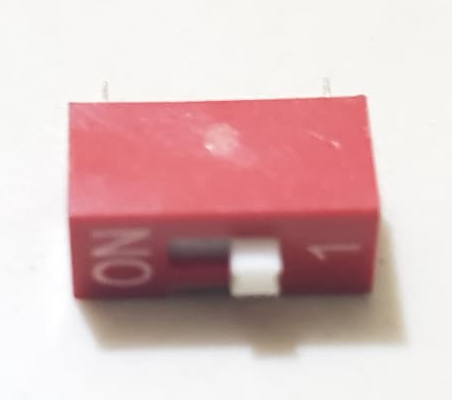
\includegraphics[height= 5cm]{Switch}
	\caption{Switch} \label{fig:switch}
\end{figure}

\subsubsection{Wires} \label{subsub:wires}

\begin{figure}[H]
	\centering
	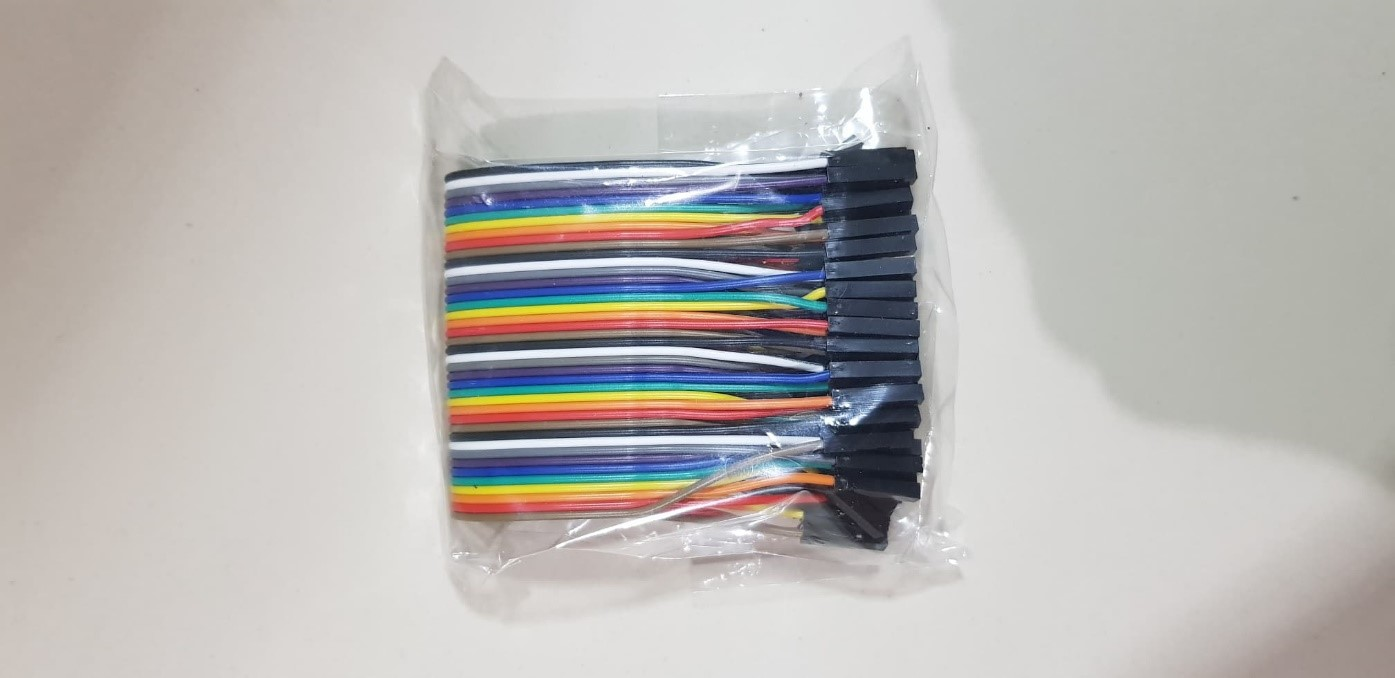
\includegraphics[height= 5cm]{Wires}
	\caption{Wires} \label{fig:wires}
\end{figure}

\subsubsection{Wheels} \label{subsub:wheels}

\begin{figure}[H]
	\centering
	\subfloat[Front Wheels.\label{fig:front}]{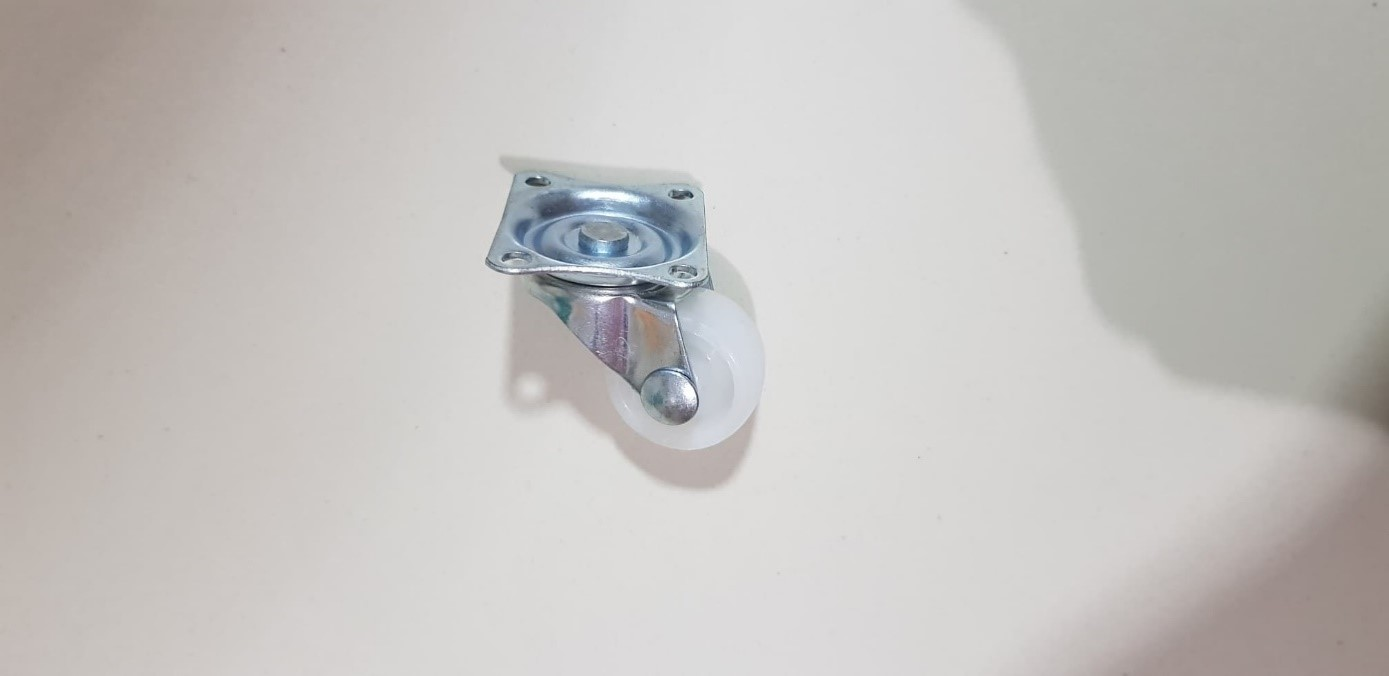
\includegraphics[height= 4cm]{Wheels2}} \hspace{0.5cm}
	\subfloat[Back Wheels.\label{fig:back}]{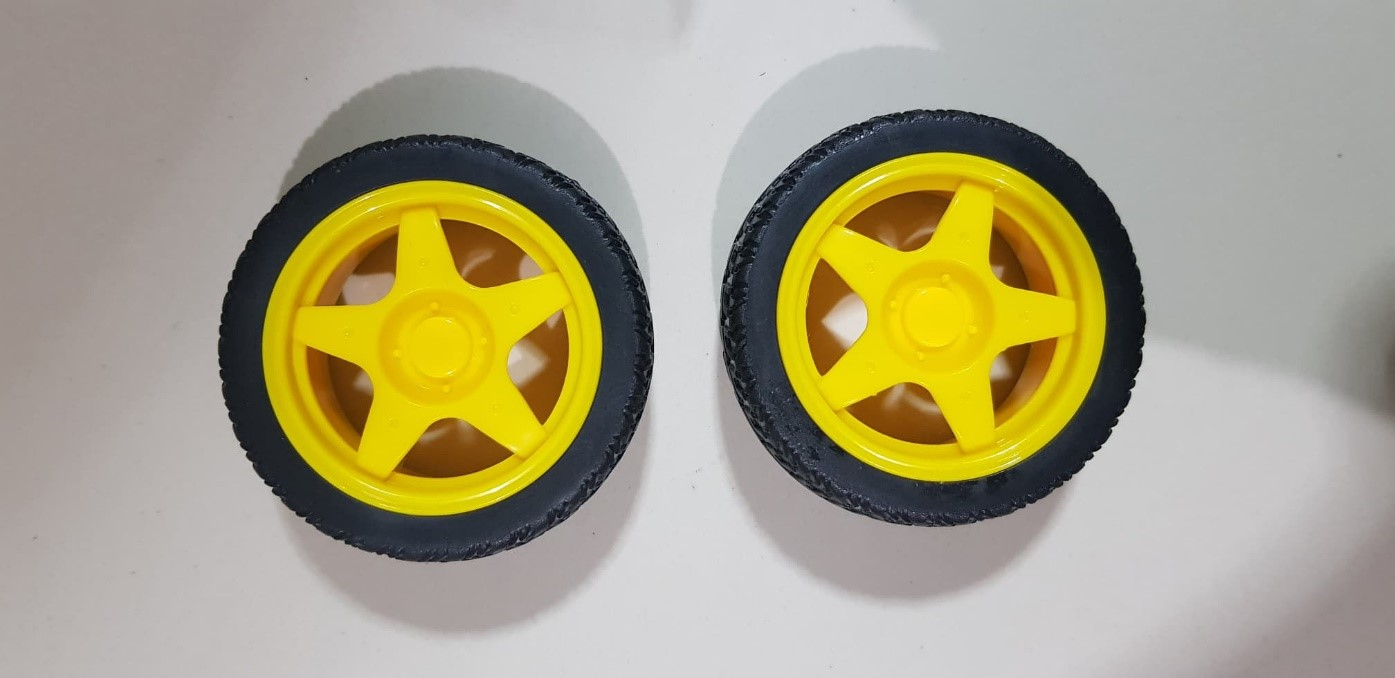
\includegraphics[height= 4cm]{Wheels1}}
	\caption{Wheels} \label{fig:wheels}
\end{figure}

\subsubsection{Batteries} \label{subsub:batteries}

\begin{figure}[H]
	\centering
	\subfloat[Batteries.\label{fig:batteries1}]{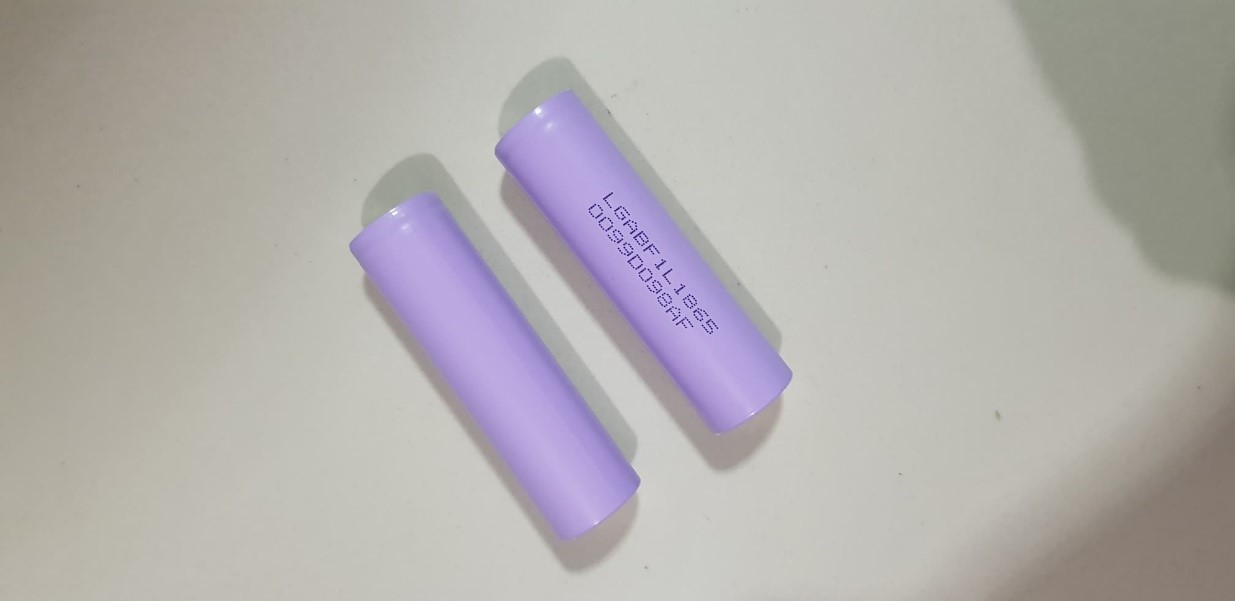
\includegraphics[height= 4cm]{Batteries1}} \hspace{0.5cm}
	\subfloat[Battery tray.\label{fig:batteries2}]{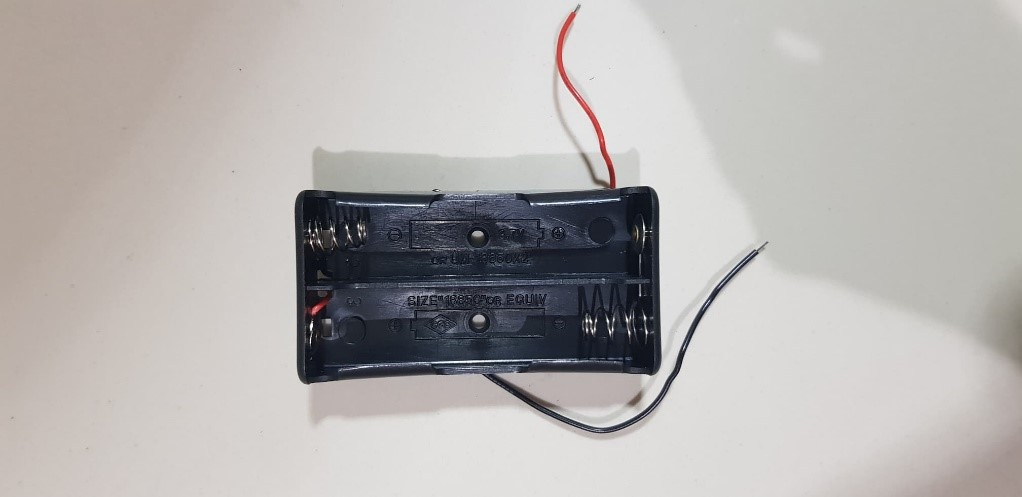
\includegraphics[height= 4cm]{Batteries2}} \\ \vspace{0.5cm}
	\subfloat[Battery charger.\label{fig:batteries3}]{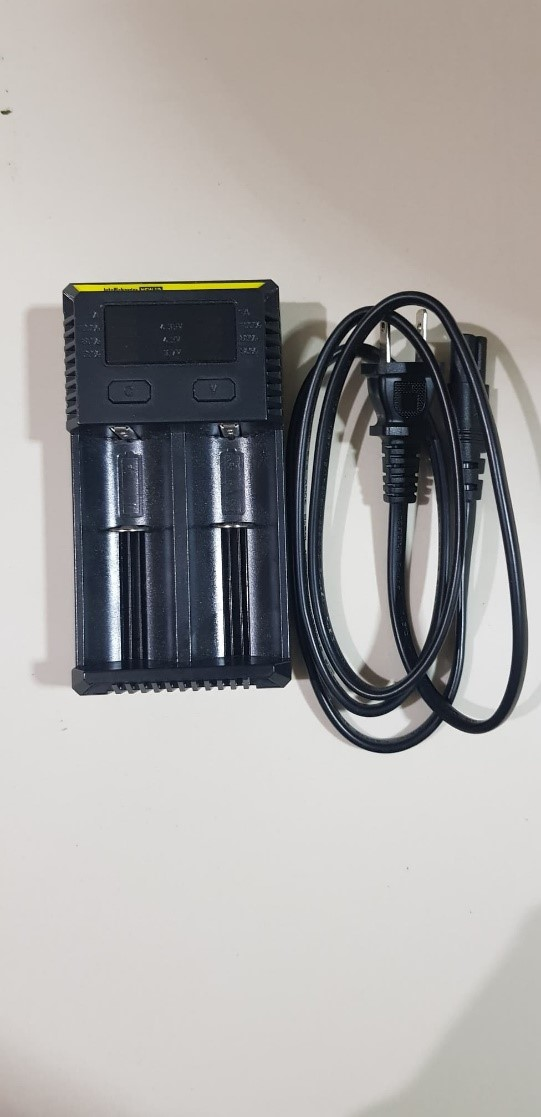
\includegraphics[height= 4cm]{Batteries3}}
	\caption{Batteries} \label{fig:batteries}
\end{figure}

\subsubsection{Magnets} \label{subsub:magnets}

\begin{figure}[H]
	\centering
	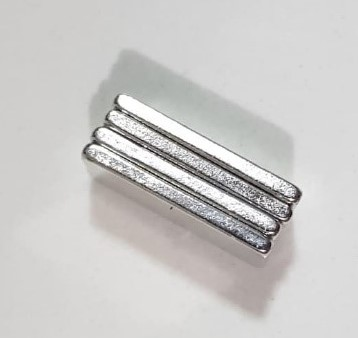
\includegraphics[height= 5cm]{Magnets}
	\caption{Magnets} \label{fig:magnets}
\end{figure}

\subsubsection{Acrylic Sheet} \label{subsub:acrylic}

\begin{figure}[H]
	\centering
	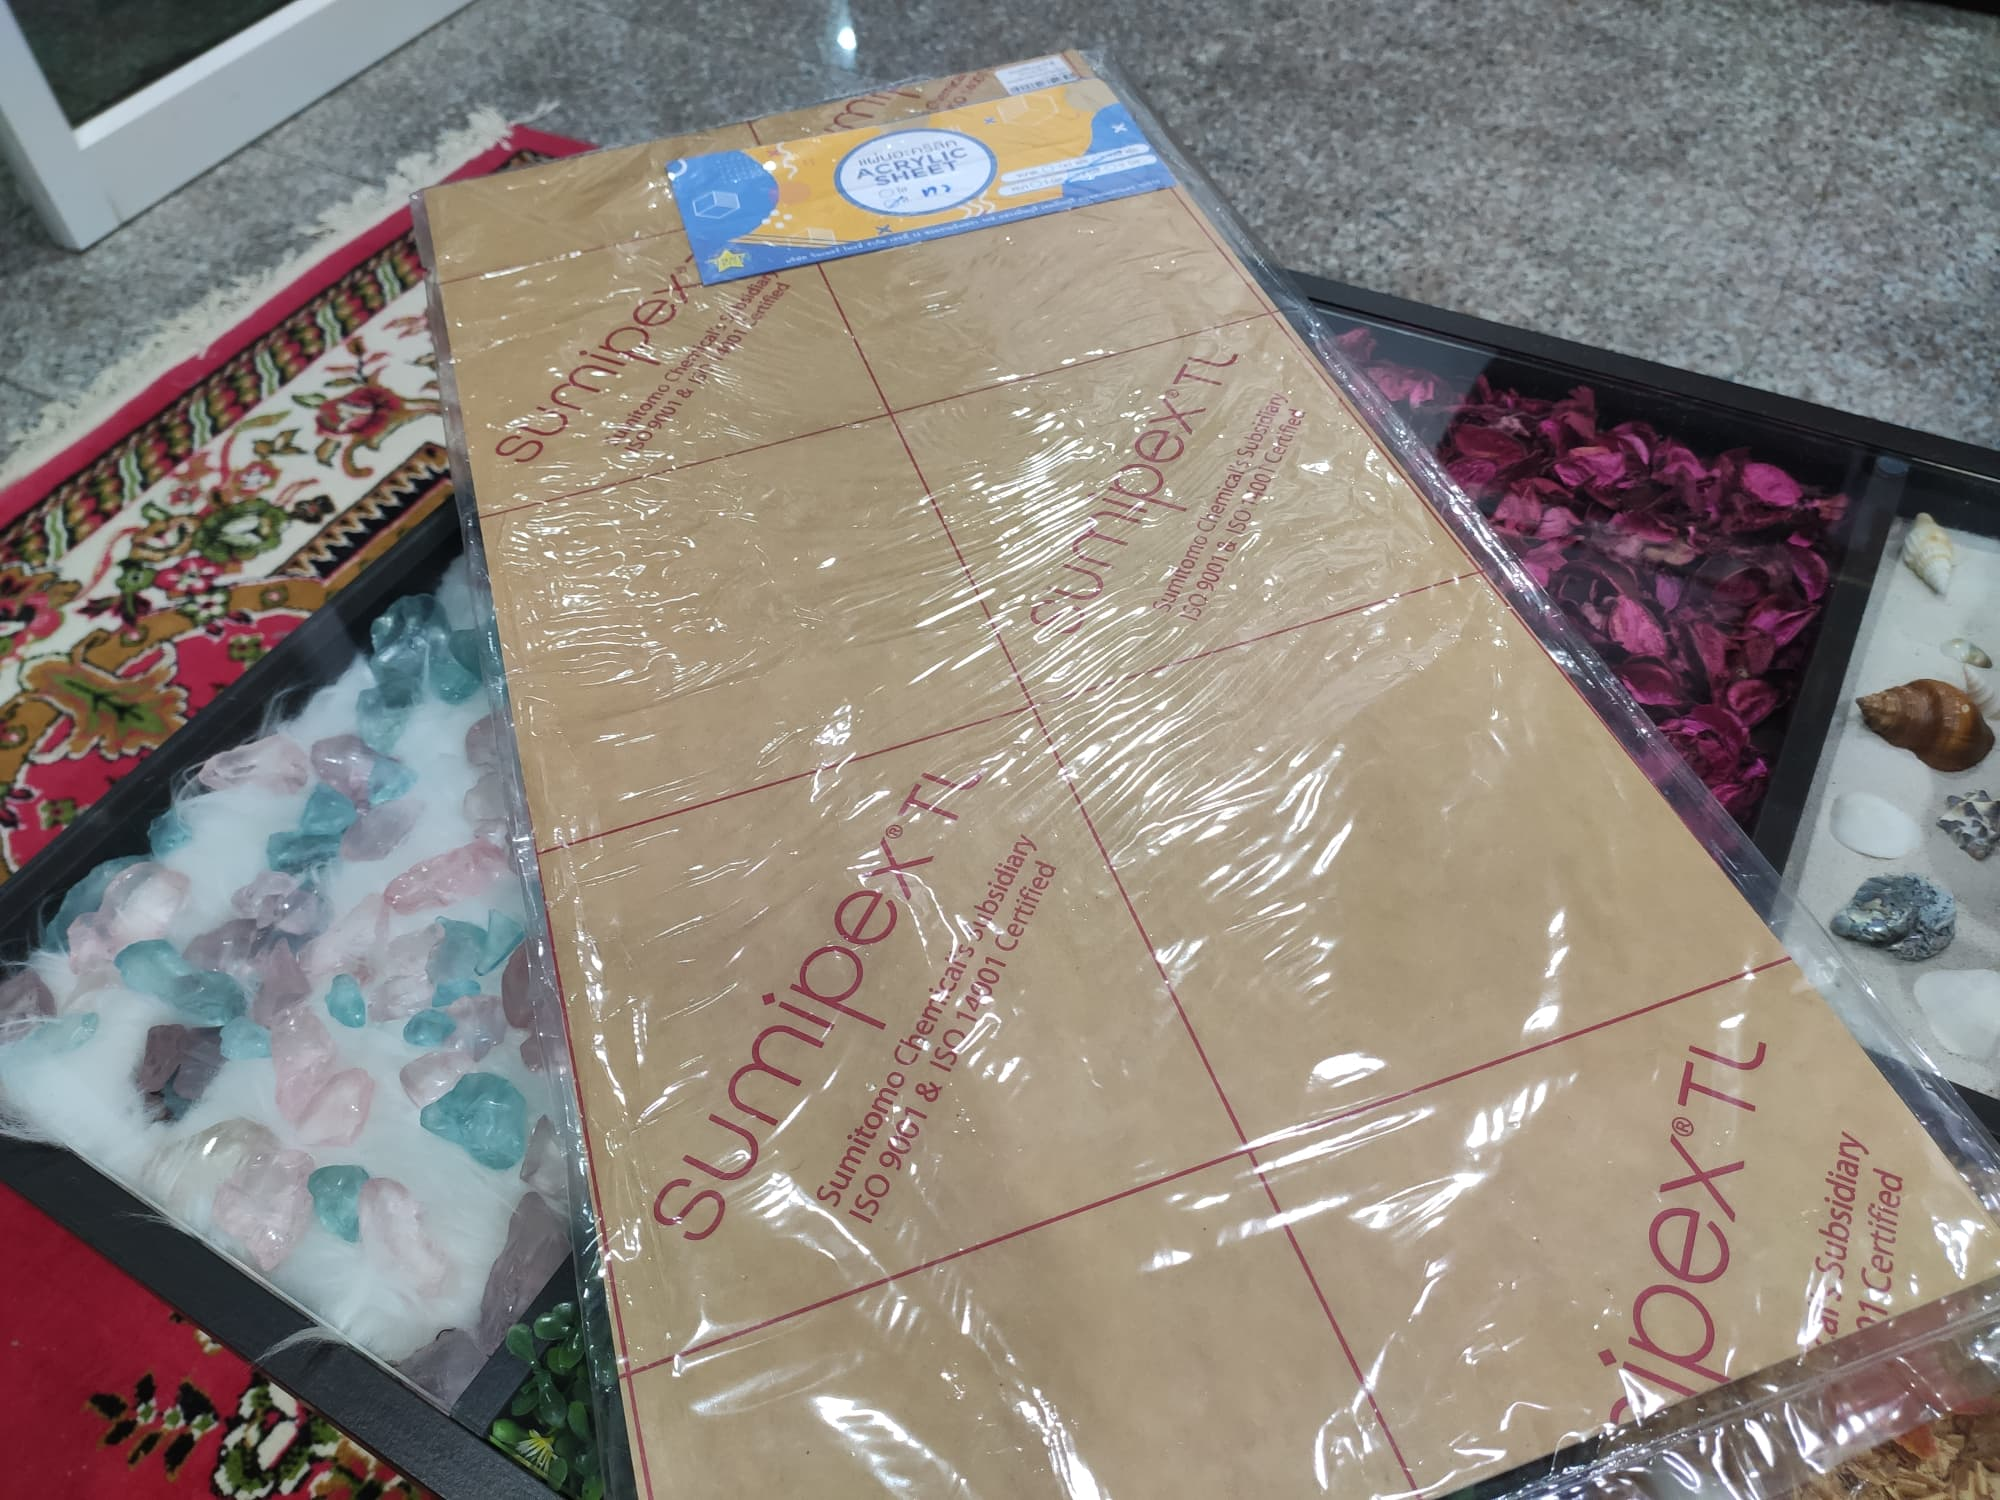
\includegraphics[height= 5cm]{Acrylic}
	\caption{Acrylic Sheet} \label{fig:acrylic}
\end{figure}

\subsubsection{Wooden Sticks} \label{subsub:sticks}

\begin{figure}[H]
	\centering
	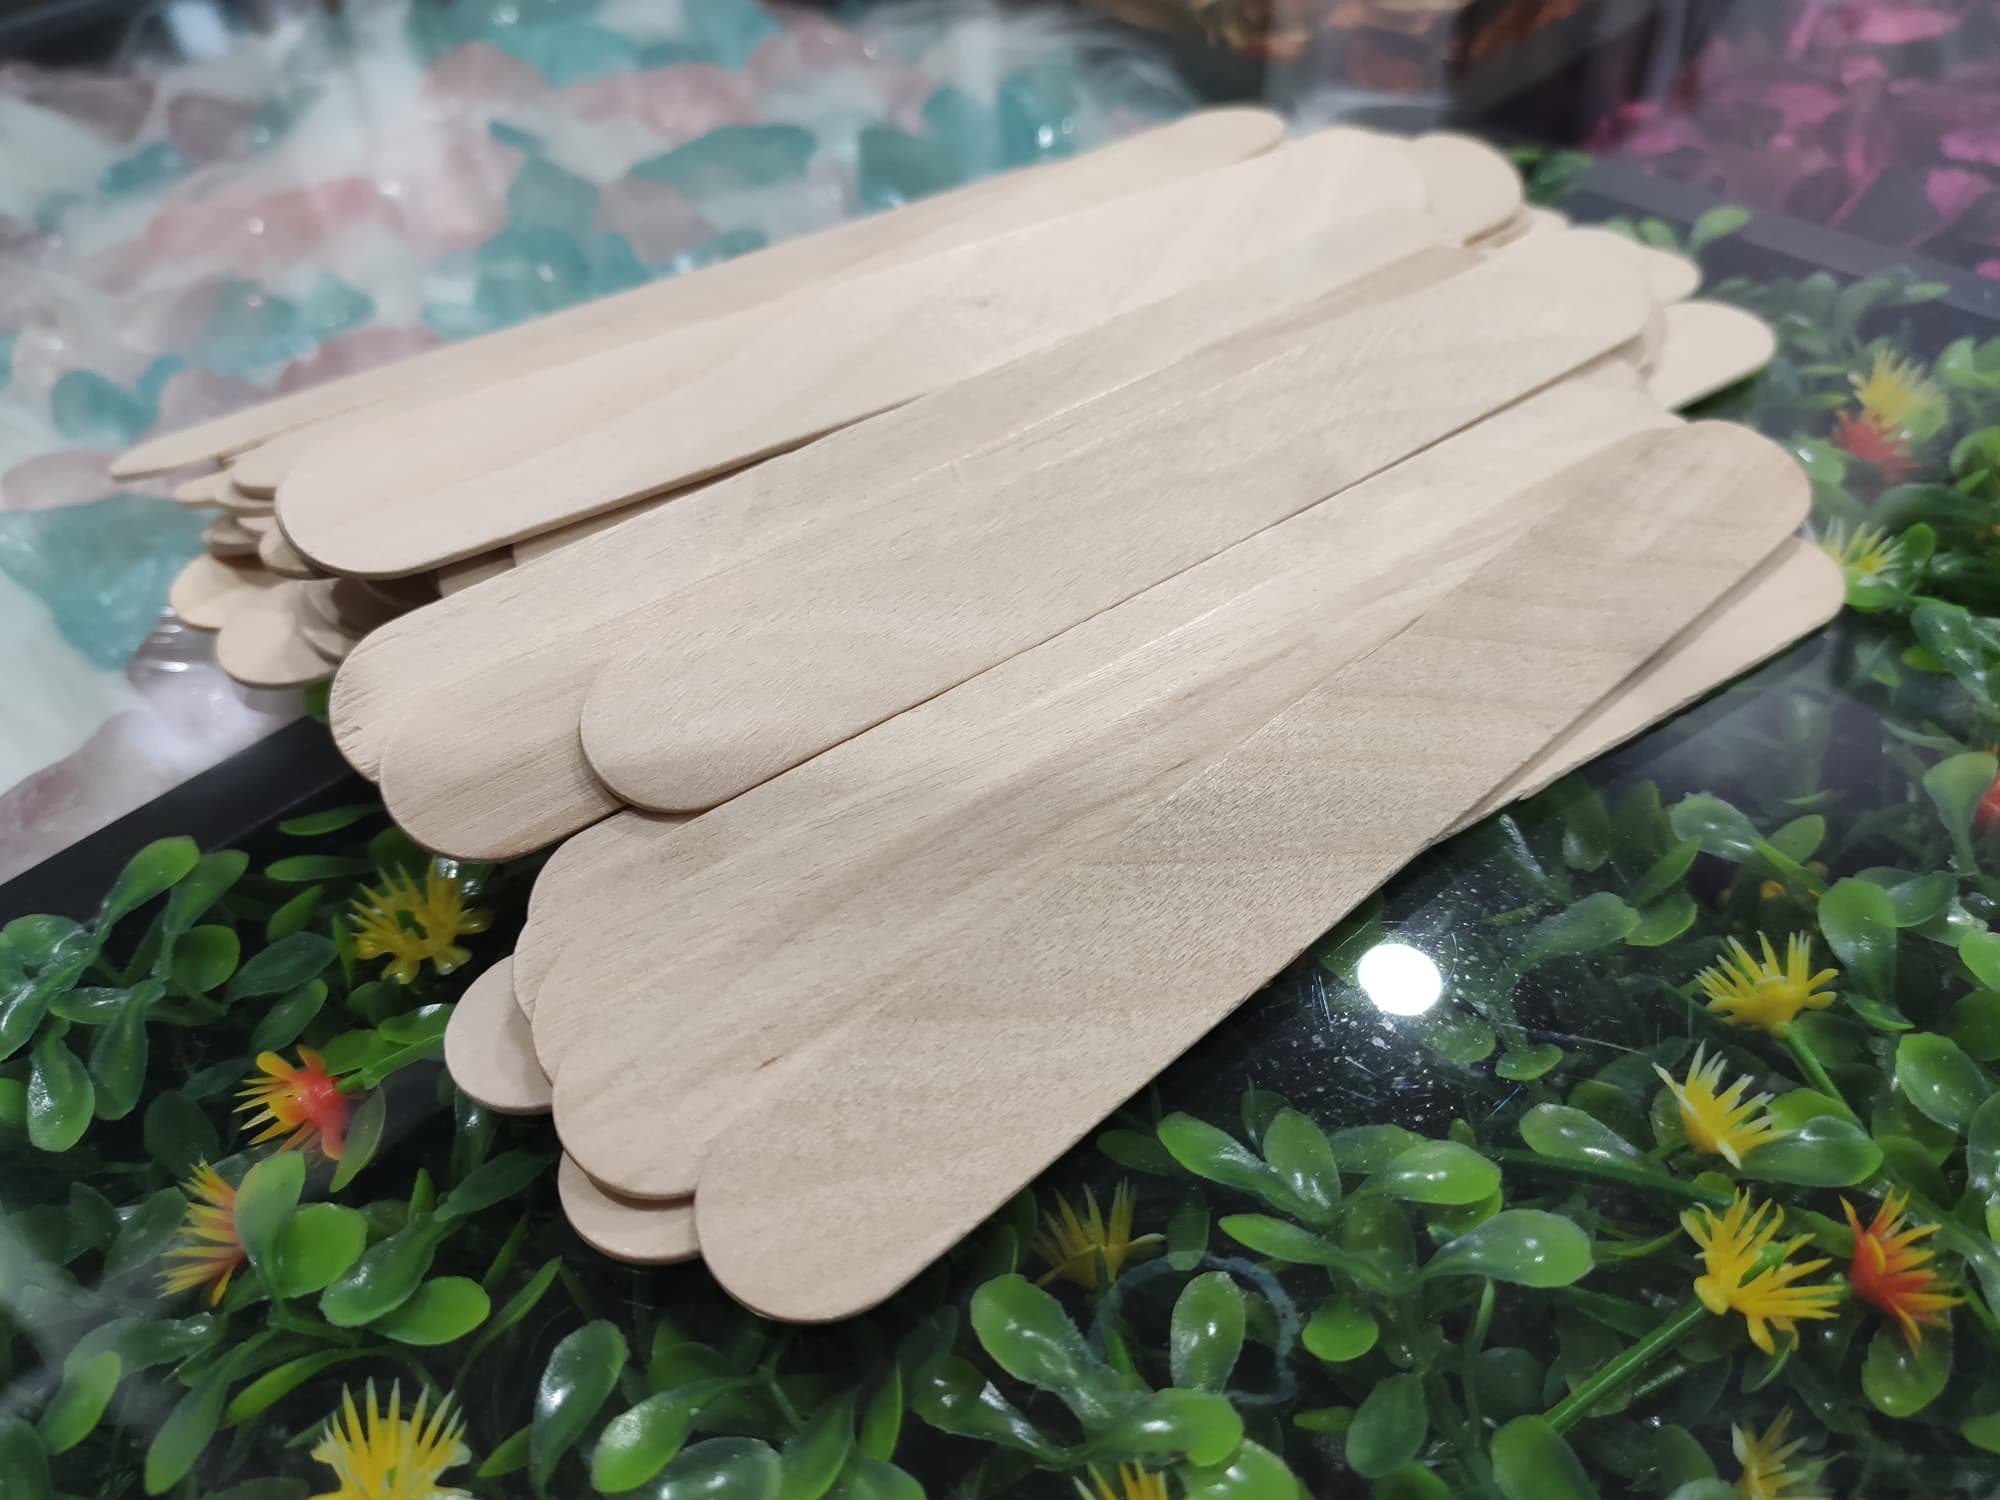
\includegraphics[height= 5cm]{Wood}
	\caption{Wooden Sticks} \label{fig:sticks}
\end{figure}

\subsubsection{Basket} \label{subsub:basket}

\begin{figure}[H]
	\centering
	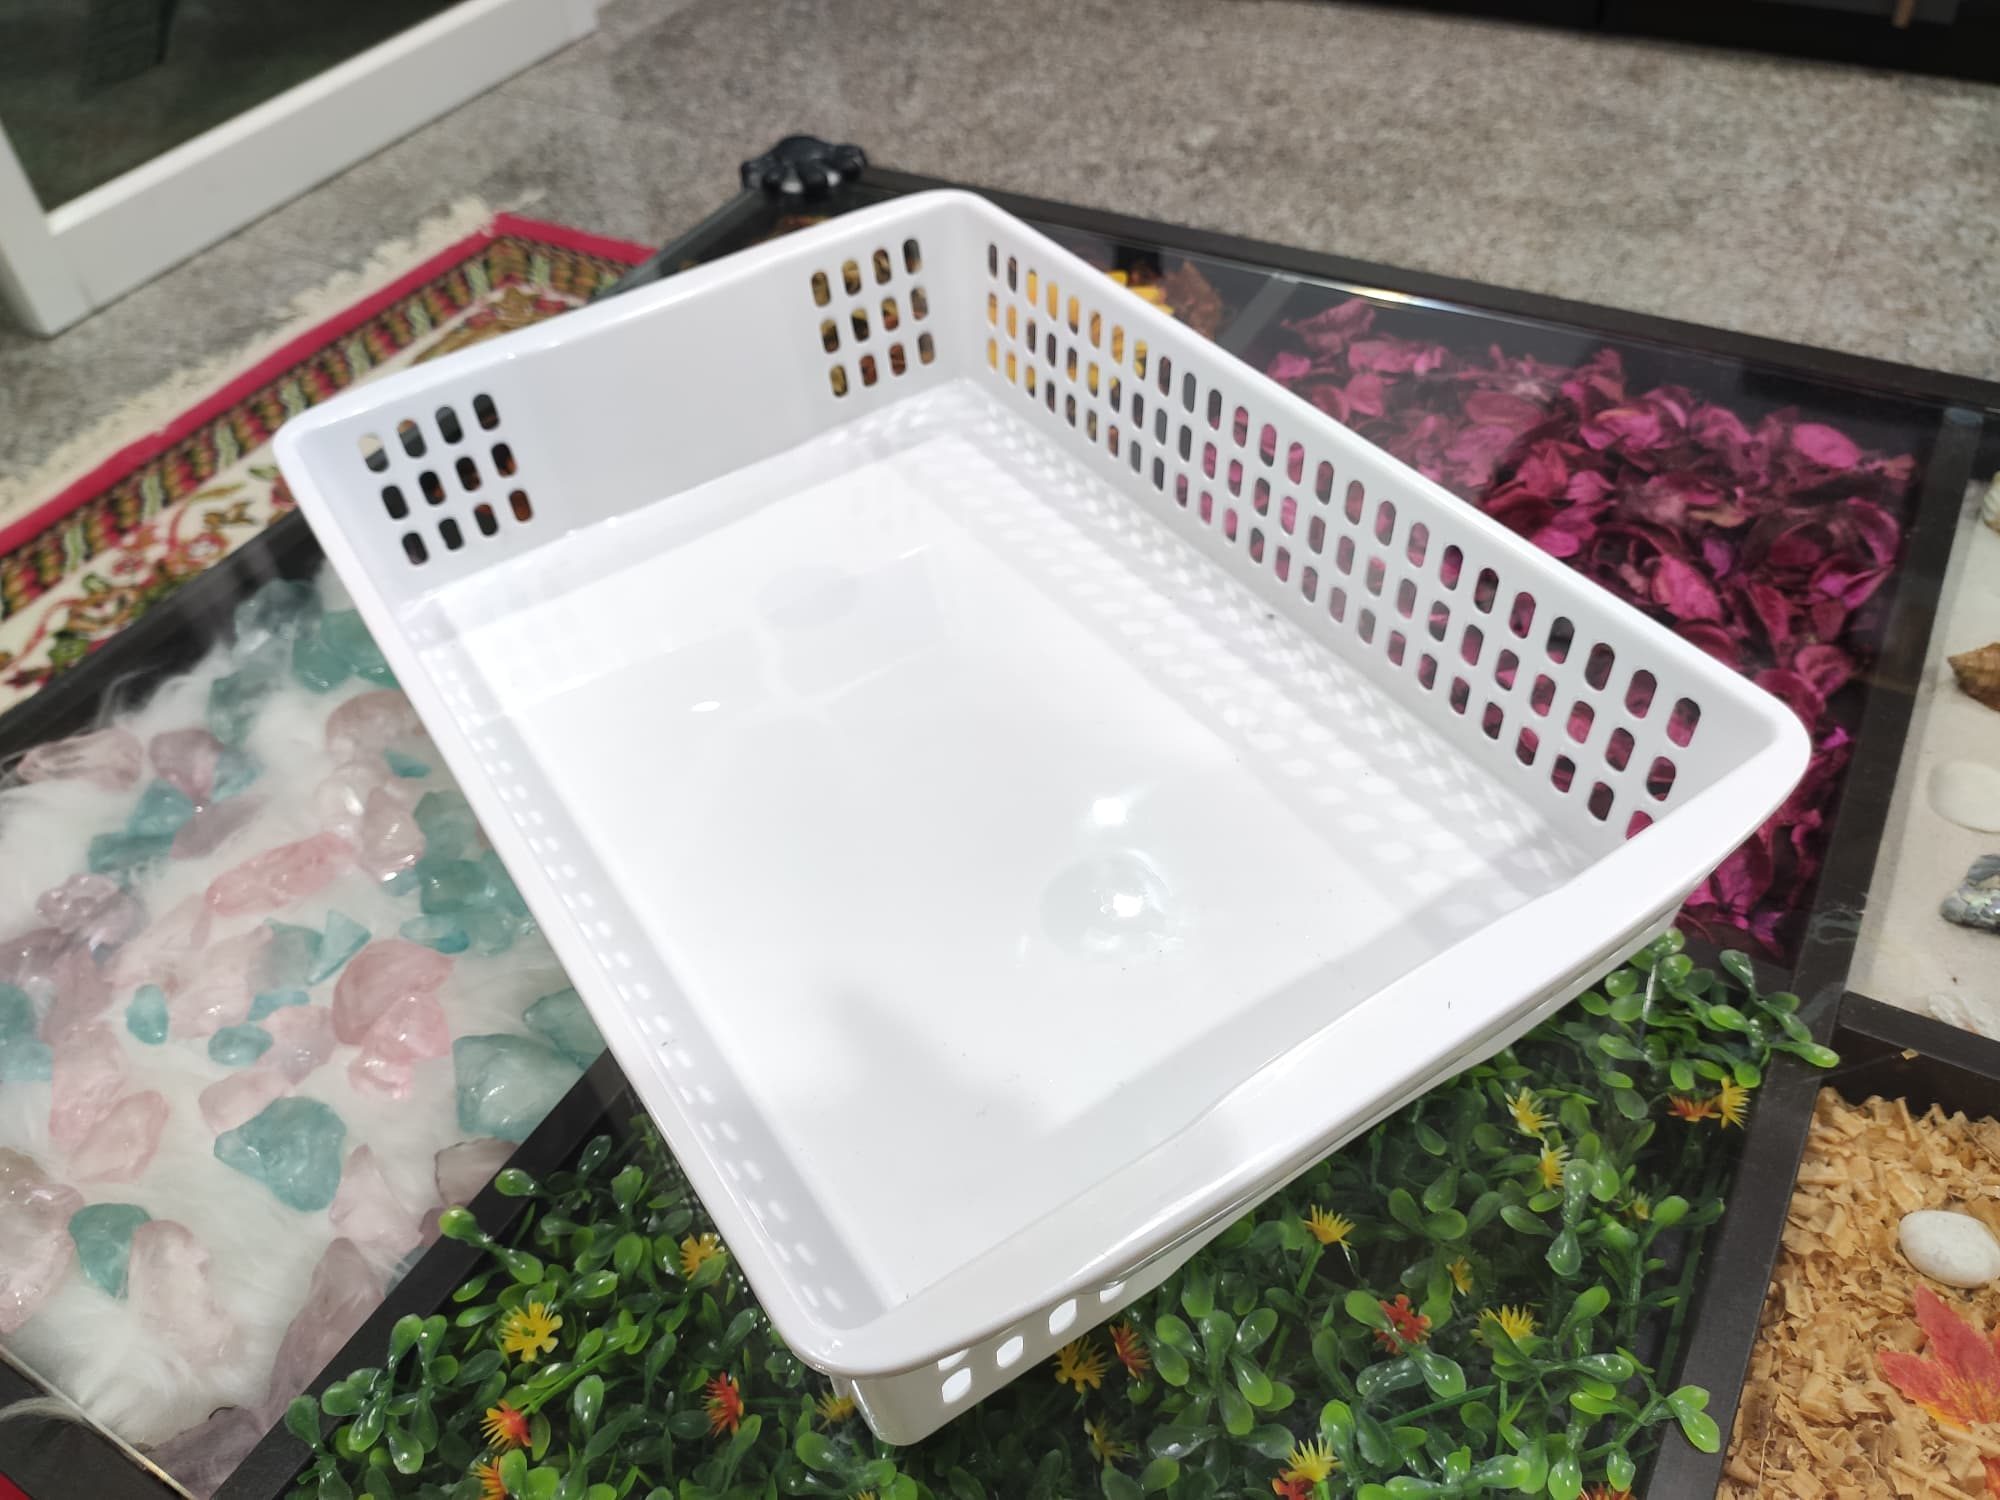
\includegraphics[height= 5cm]{Basket}
	\caption{Basket} \label{fig:basket}
\end{figure}

\subsubsection{Solderless Bread Board} \label{subsub:breadboard}

\begin{figure}[H]
	\centering
	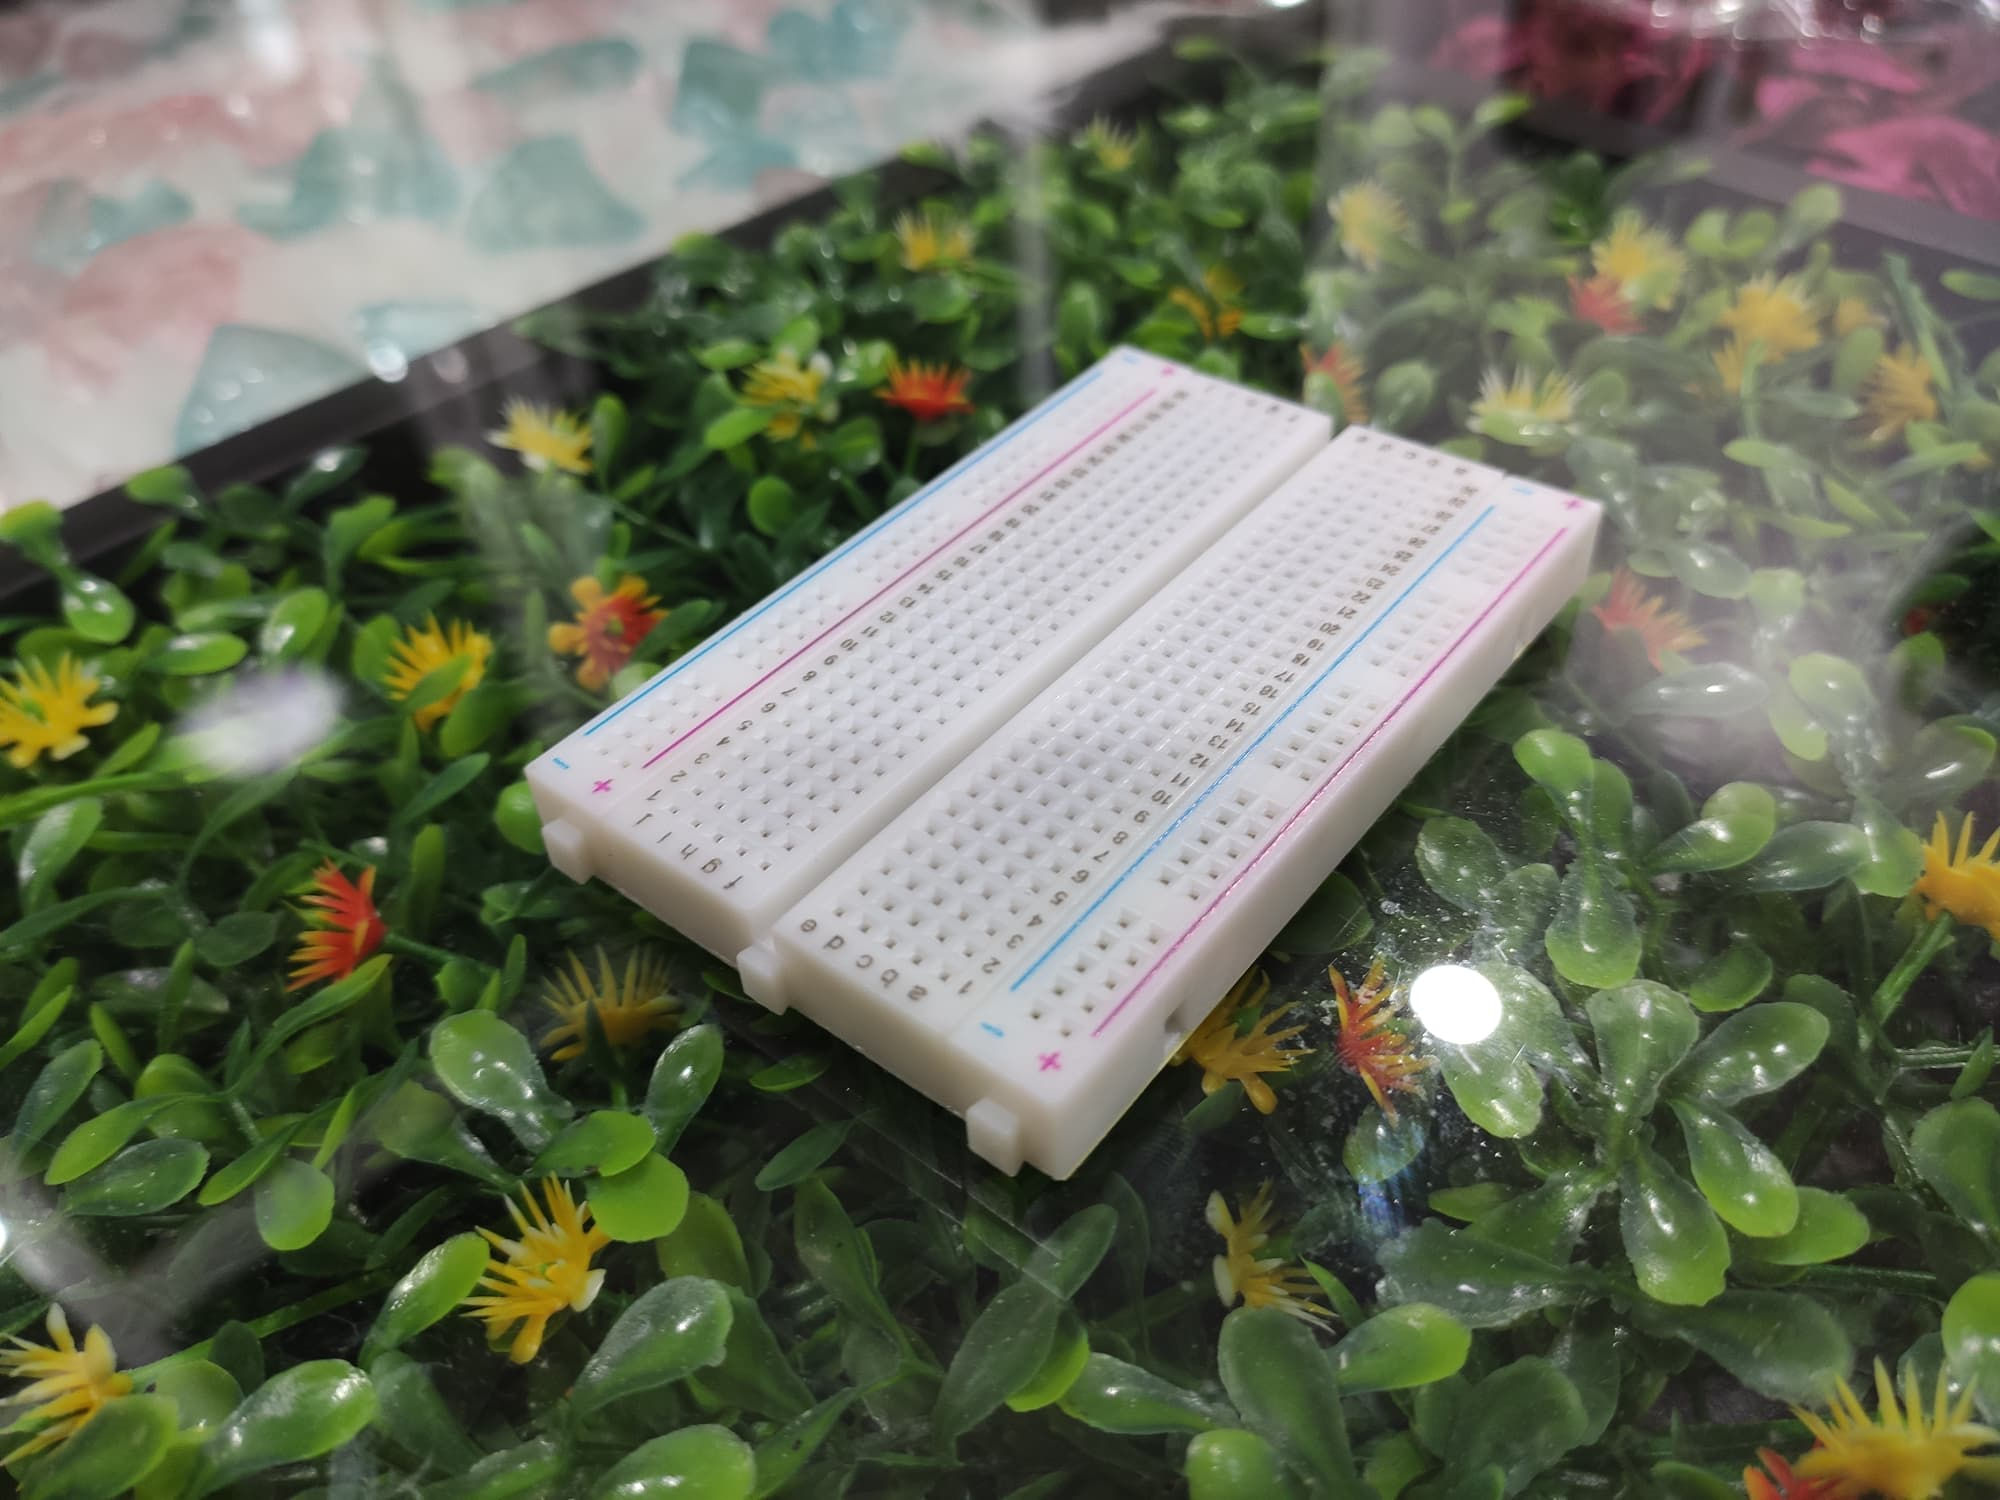
\includegraphics[height= 5cm]{Breadboard}
	\caption{Solderless Bread Board} \label{fig:breadboard}
\end{figure}

\subsubsection{Stud bolt and Nut} \label{subsub:stud}

\begin{figure}[H]
	\centering
	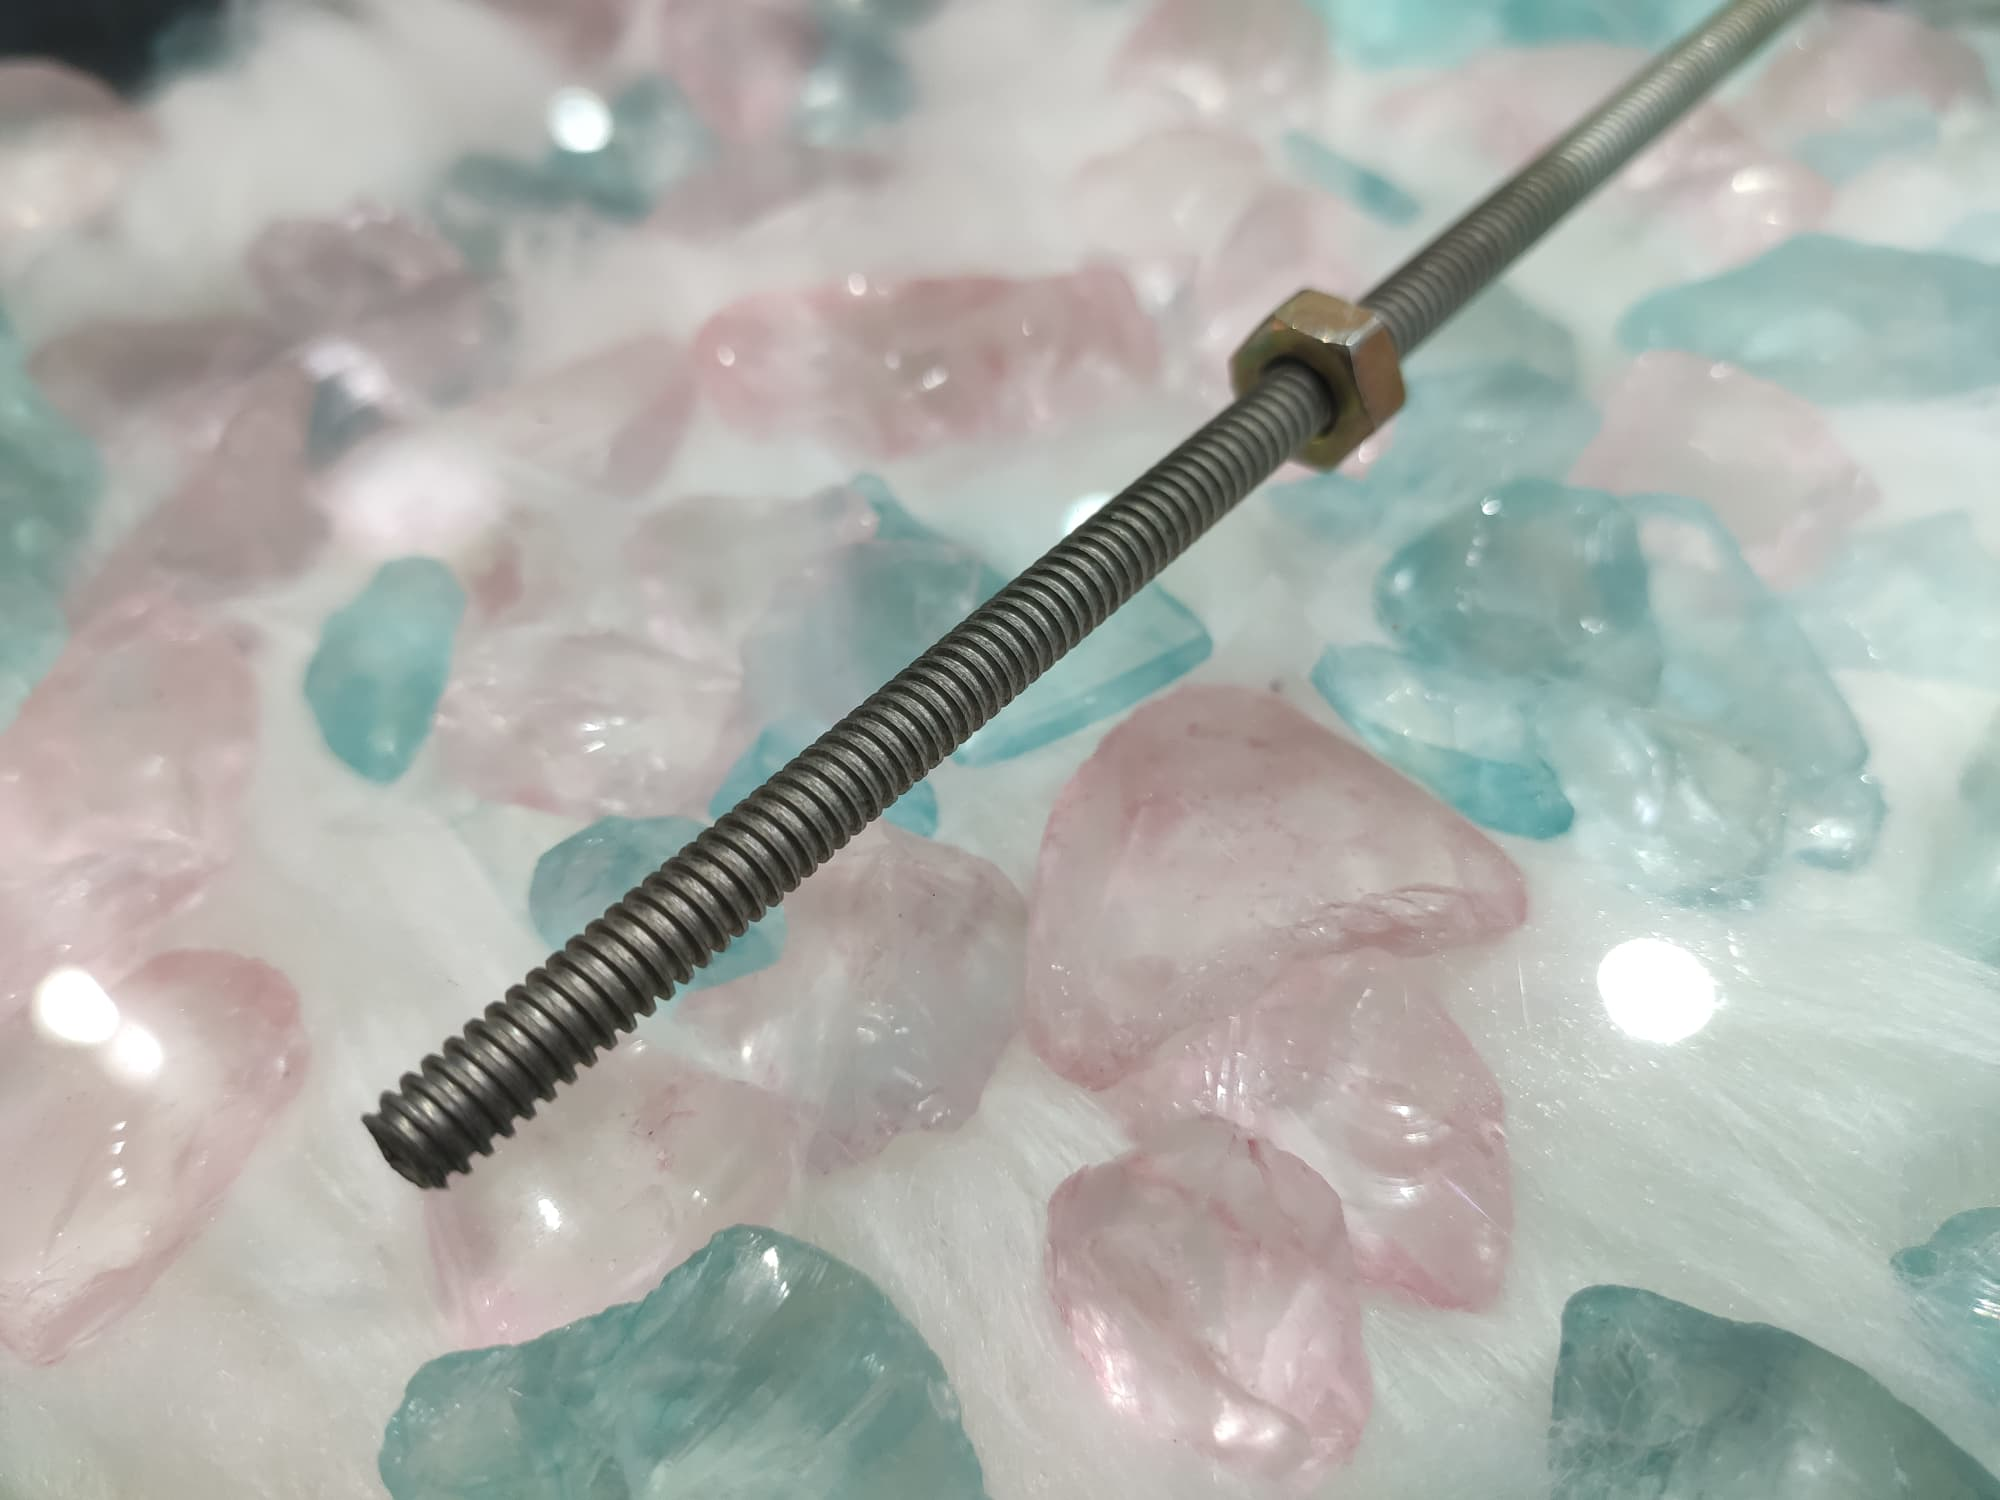
\includegraphics[height= 5cm]{Stud}
	\caption{Stud bolt and Nut} \label{fig:stud}
\end{figure}


\subsection{Mechanism Design of the system} \label{sub:mechanism}

\begin{figure}[H]
	\centering
	\subfloat[Expected 3D Design of the system.\label{fig:design1}]{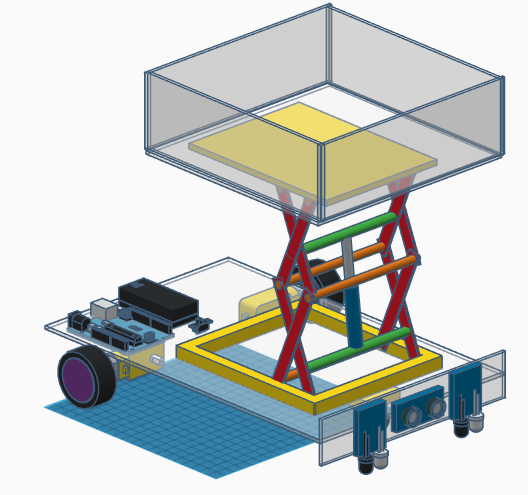
\includegraphics[height= 5cm]{Design1}} \hspace{1cm}
	\subfloat[Expected 3D Design of the system.\label{fig:design2}]{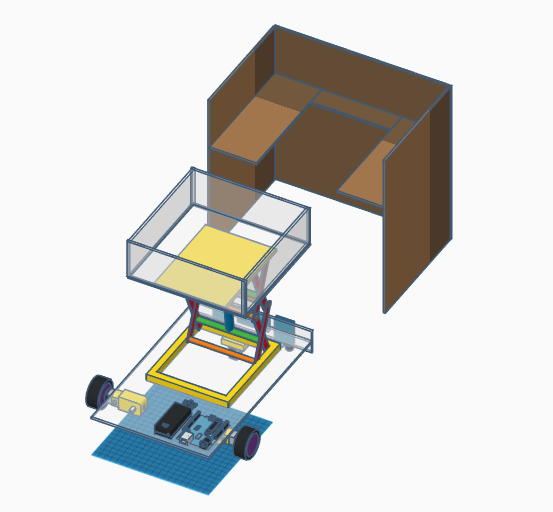
\includegraphics[height= 5cm]{Design2}}
	\caption{3D design of DIY Automatic Delivery Trolley and stations.} \label{fig:3ddesign}
\end{figure}

As we see in Figure \ref{fig:3ddesign}, the finishing product is anticipated to be driven by the motors and has the direction controlled by the IR sensor which has Arduino UNO as a compute center. Moreover, there will be a scissor lift to deliver the document to the hand of the sender (in sit position).

\subsection{Circuit diagram of DIY Automatic Delivery Trolley} \label{sub:circuit}

\begin{center}
	\textcolor{red}{In Progress}
\end{center}

\subsection{Flow chart of the system}

\begin{figure}[H]
	\centering
	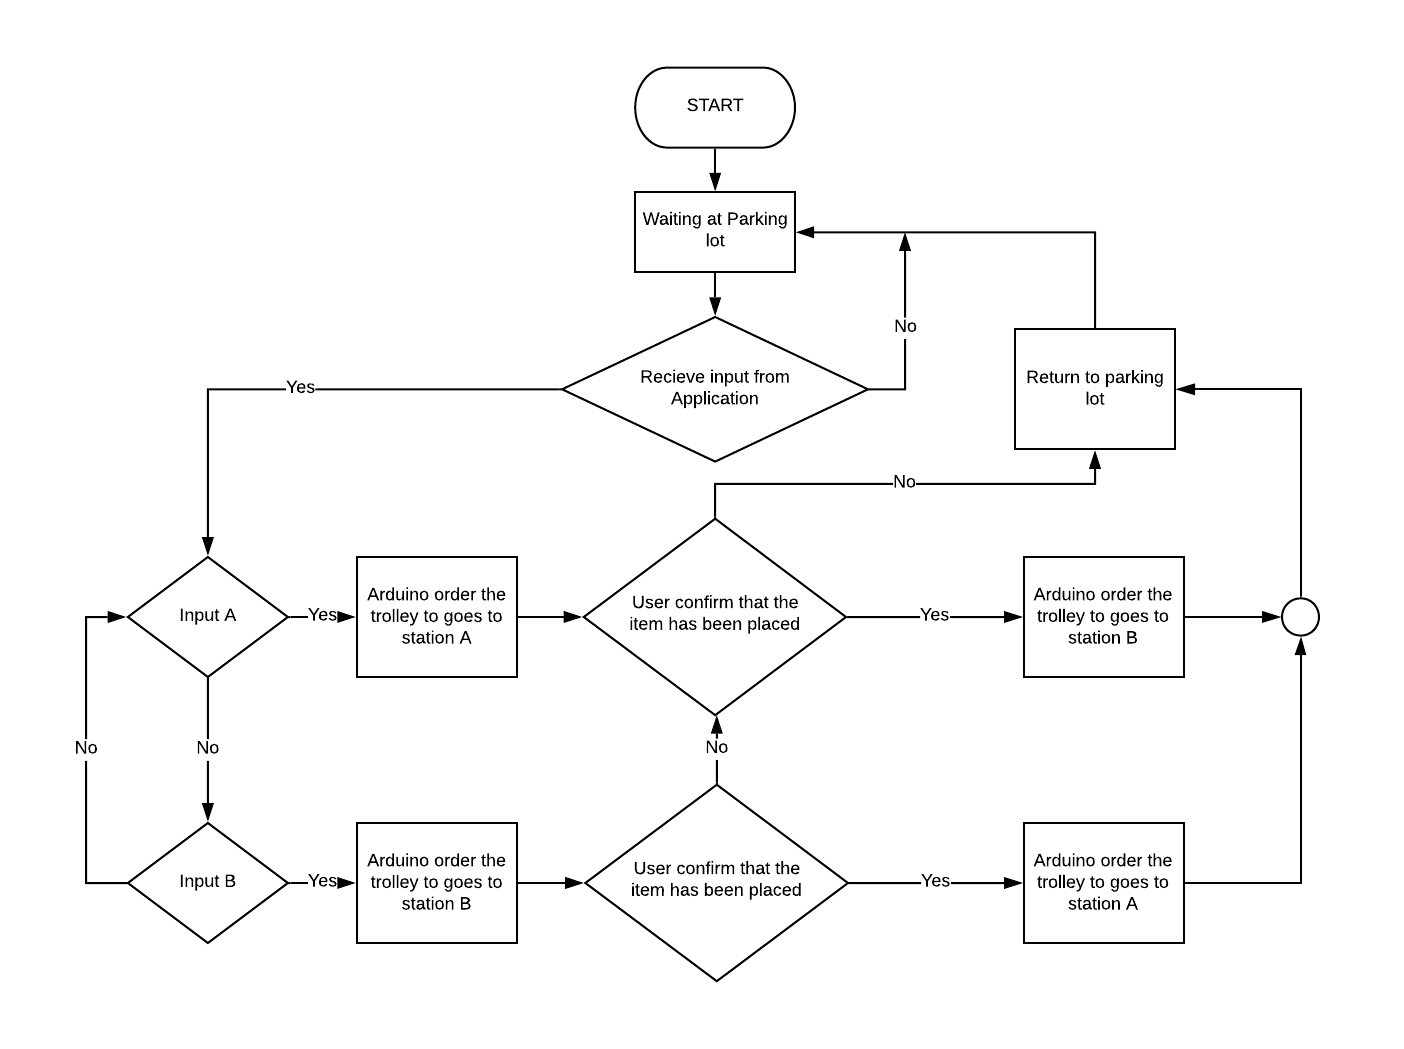
\includegraphics[height= 13cm]{Flowchart}
	\caption{Flow chart of the system} \label{fig:flowchart}
\end{figure}

As shown in Figure \ref{fig:flowchart}, our trolley will wait at the parking spot. When it receives order from the application, they will go to the station according to the input which are input A goes to station A and input B goes to station B. The trolley will wait at the station for the user to confirm that the document has been placed at amount of time. If there is no confirmation, the trolley will return to the station. When the user has confirmed, the trolley will deliver the document to another station and then it will return to the parking spot and wait for another order.

\section{Methology} \label{sec:methology}

In this section we will guild you how can we build the DIY trolley. \par
Firstly, all electronics were checked whether it is broken or not.

\begin{figure}[H]
	\centering
	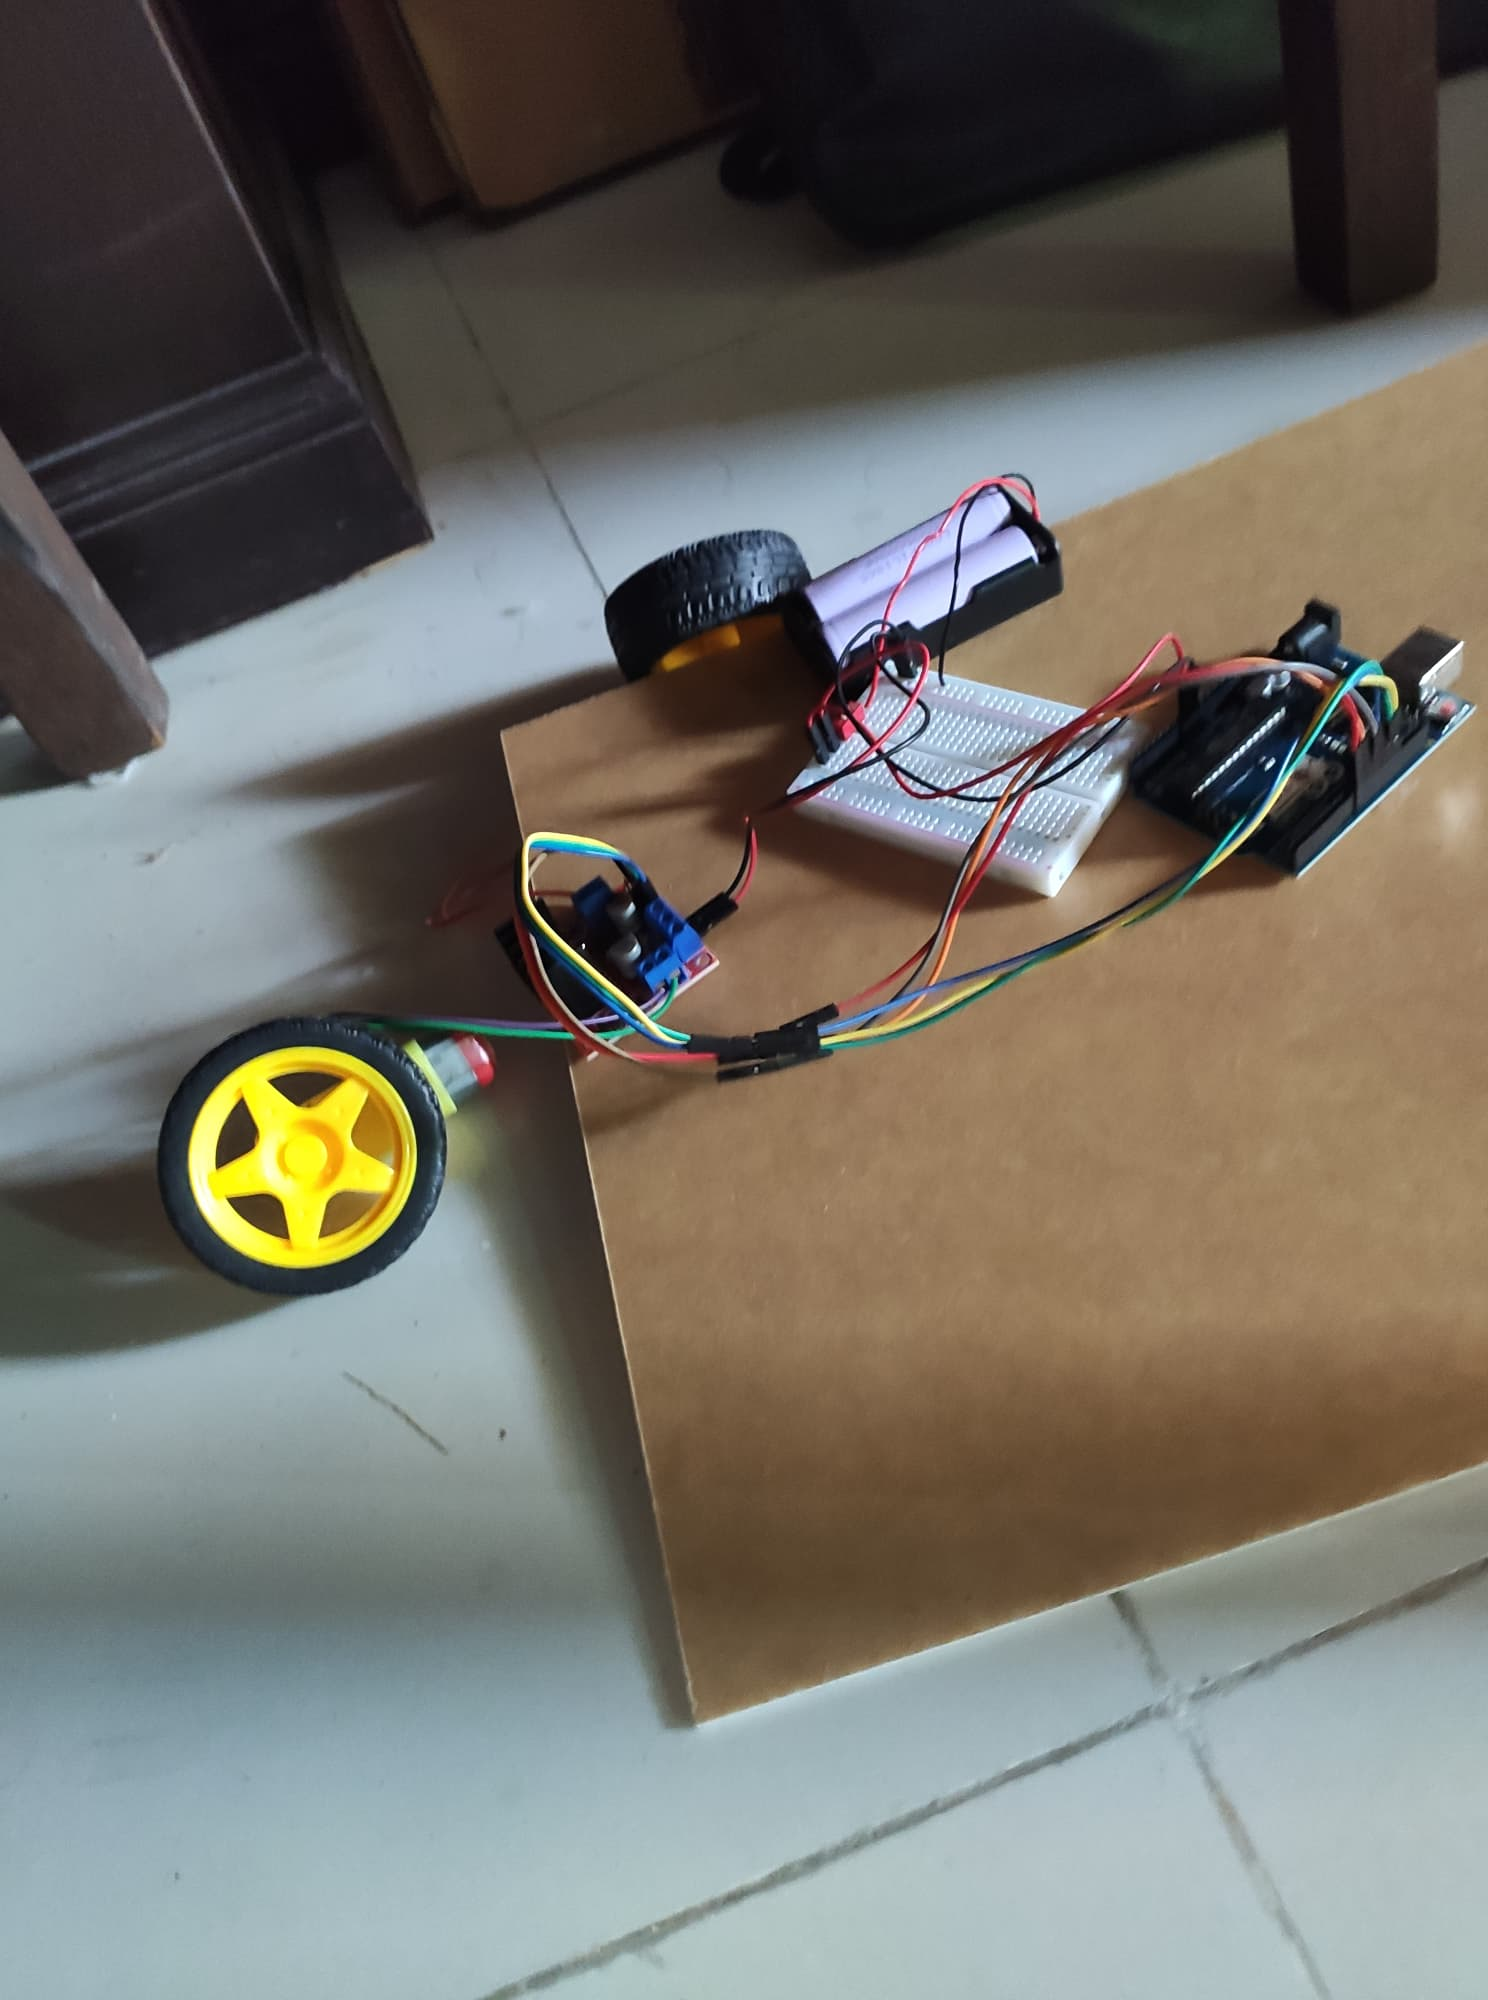
\includegraphics[height= 5cm]{M1}
	\caption{All electronics were checked} \label{fig:m1}
\end{figure}

\par 

Secondly, the motors and wheels were attached to the acrylic.

\begin{figure}[H]
	\centering
	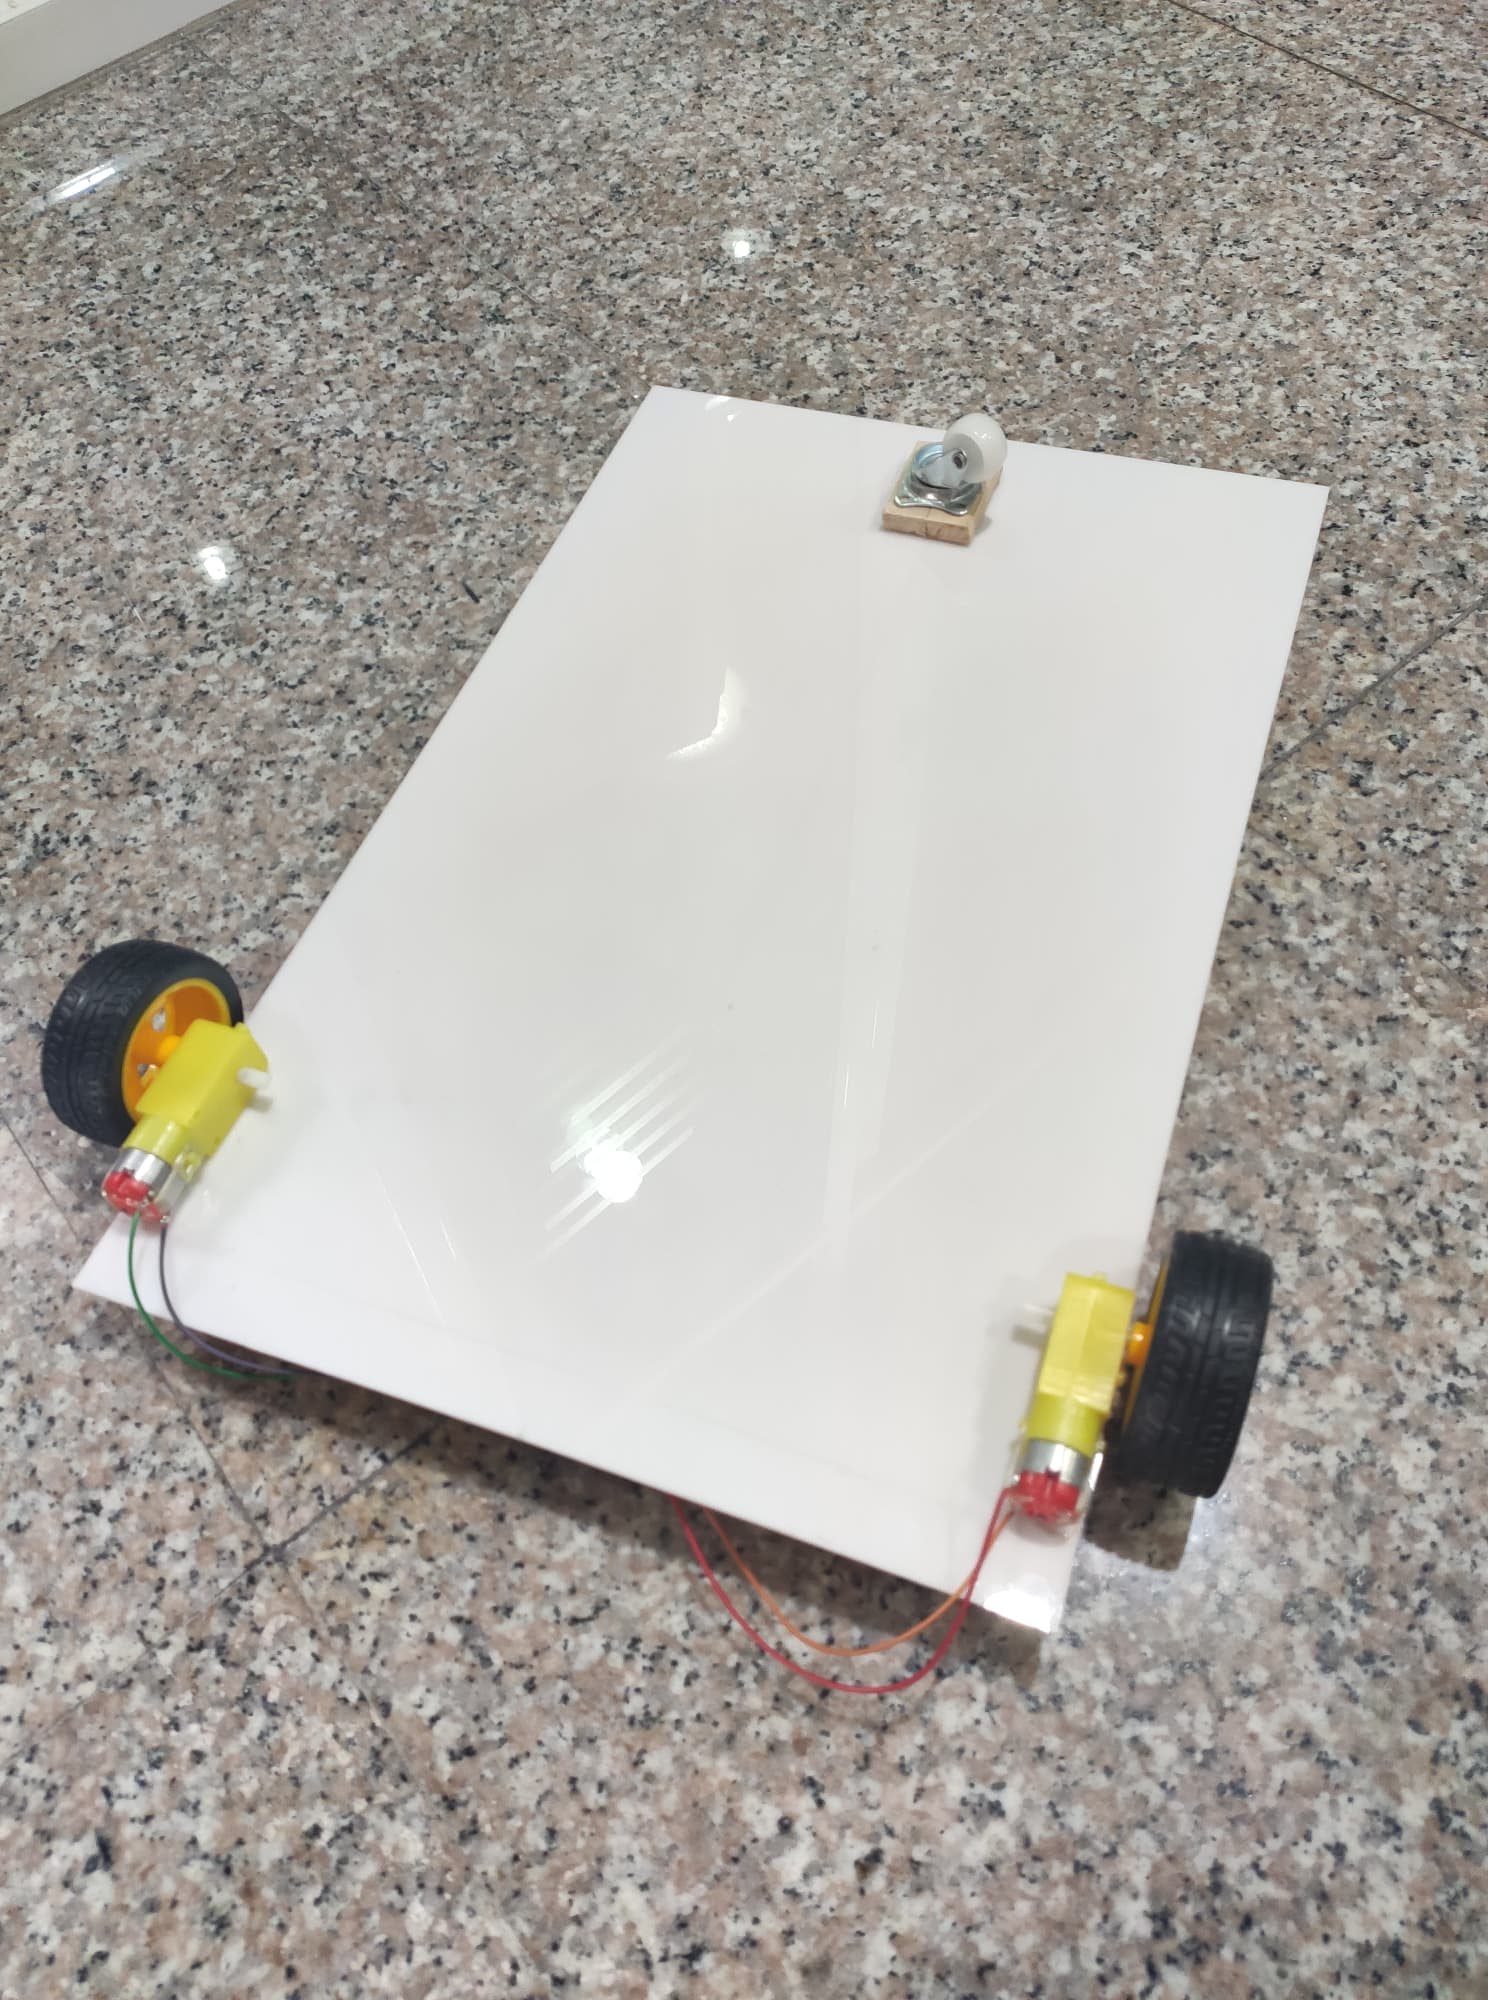
\includegraphics[height= 5cm]{M2}
	\caption{The motors and wheels were attached to the acrylic} \label{fig:m2}
\end{figure}

\par

Thirdly, the acrylic was reinforced with polycarbonate and motors were fortify with aluminum.

\begin{figure}[H]
	\centering
	\subfloat[Polycarbonate \label{fig:m3}]{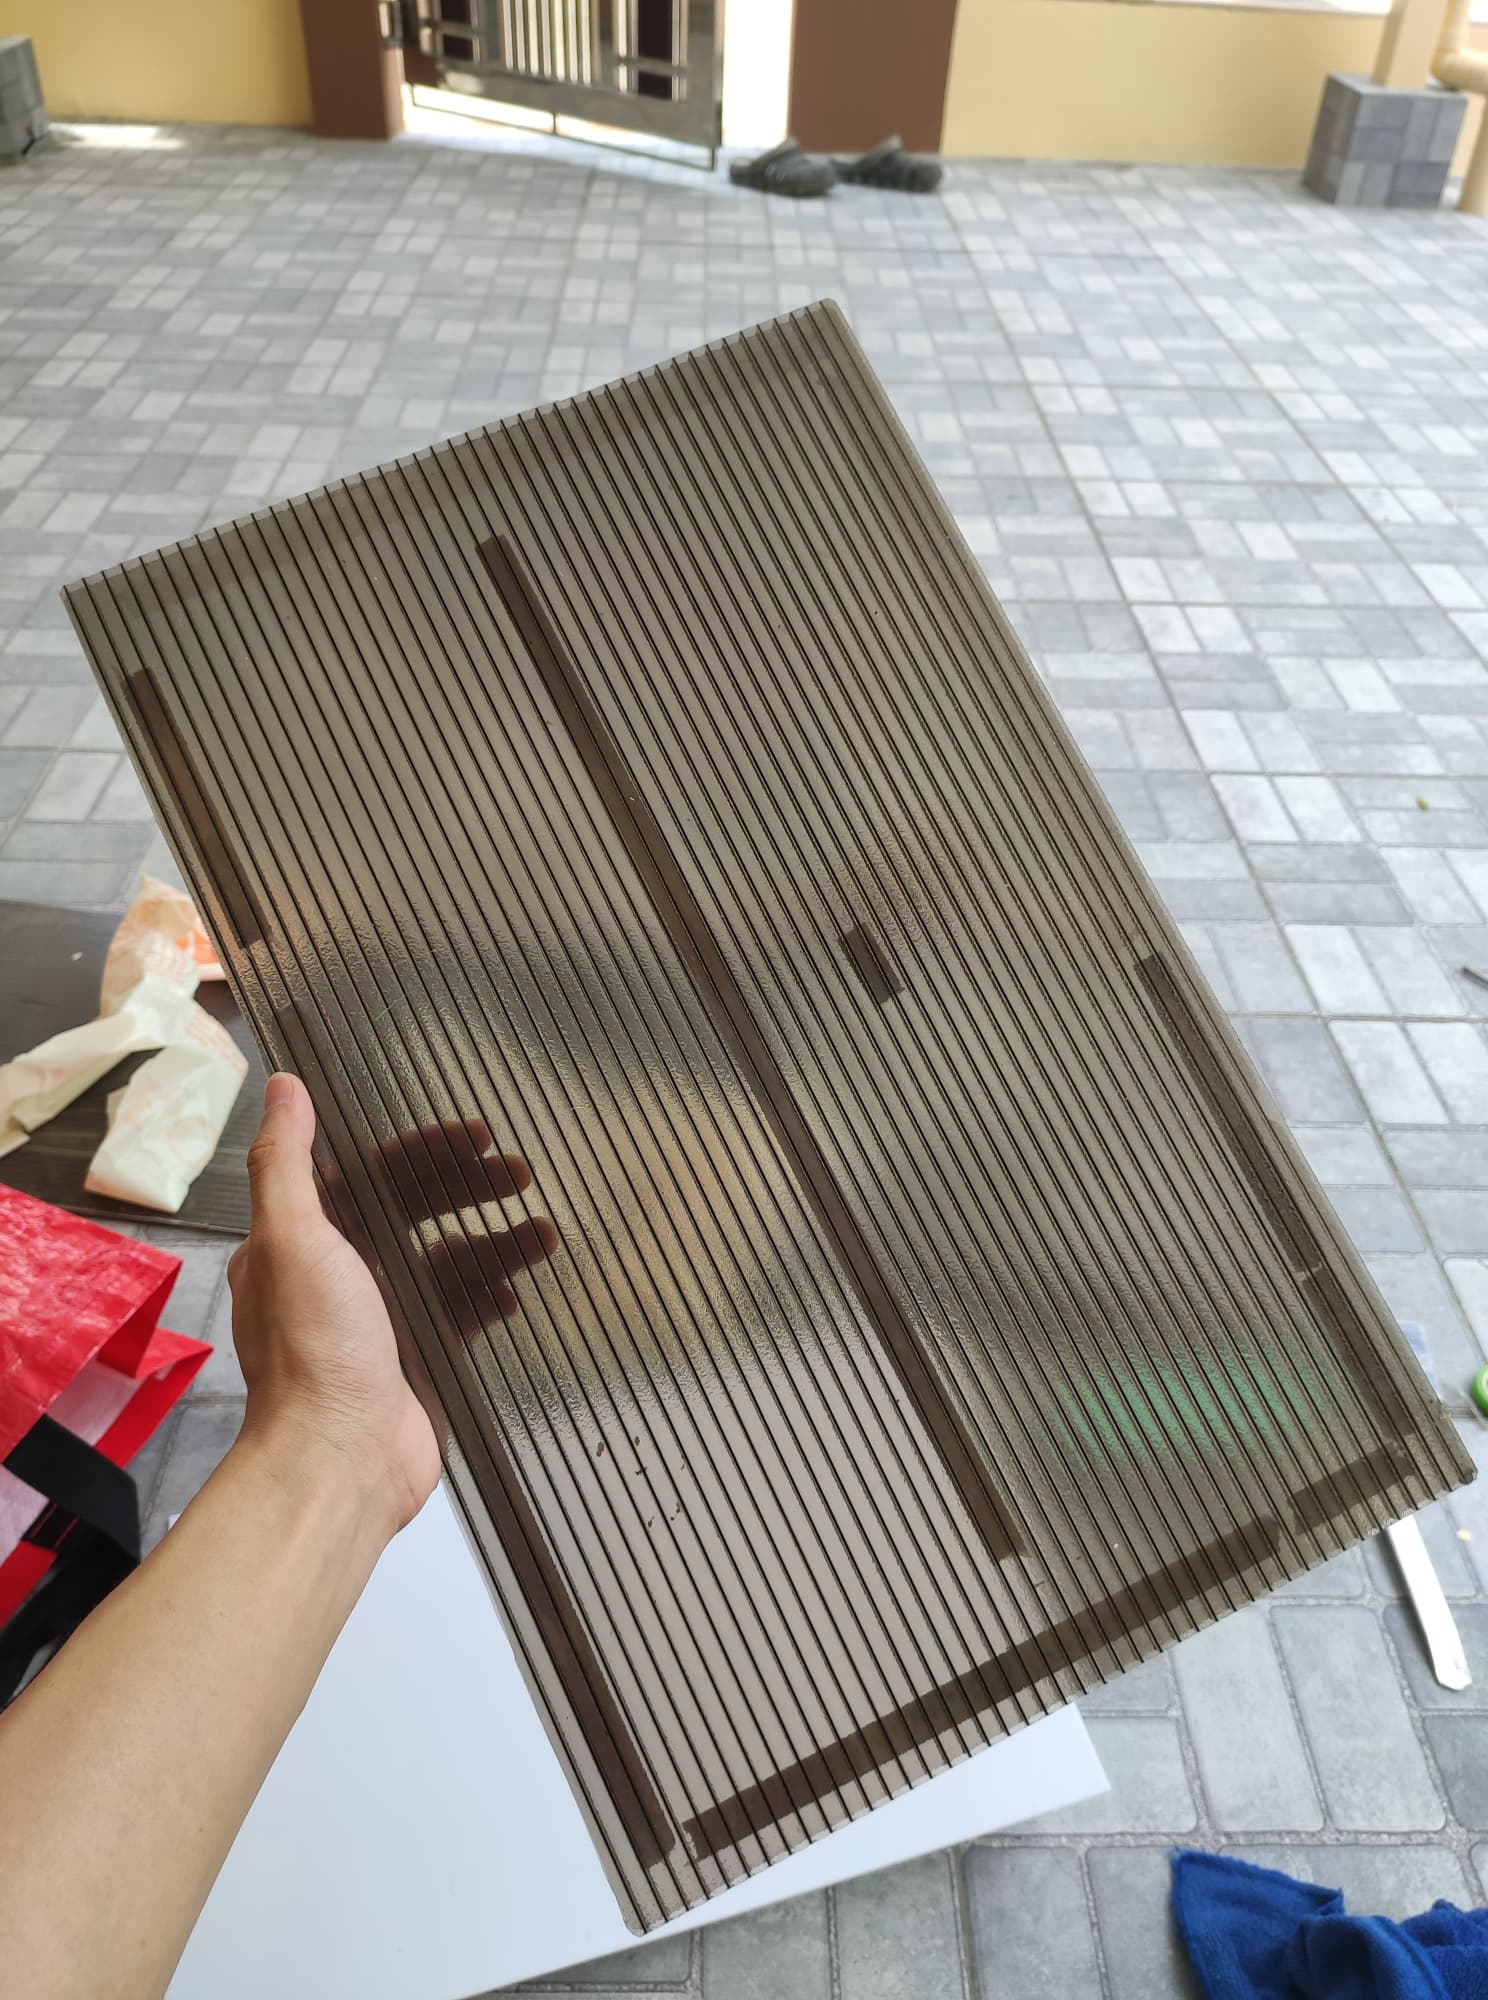
\includegraphics[height= 5cm]{M3}} \hspace{1cm}
	\subfloat[Motors were fortify with aluminum \label{fig:m4}]{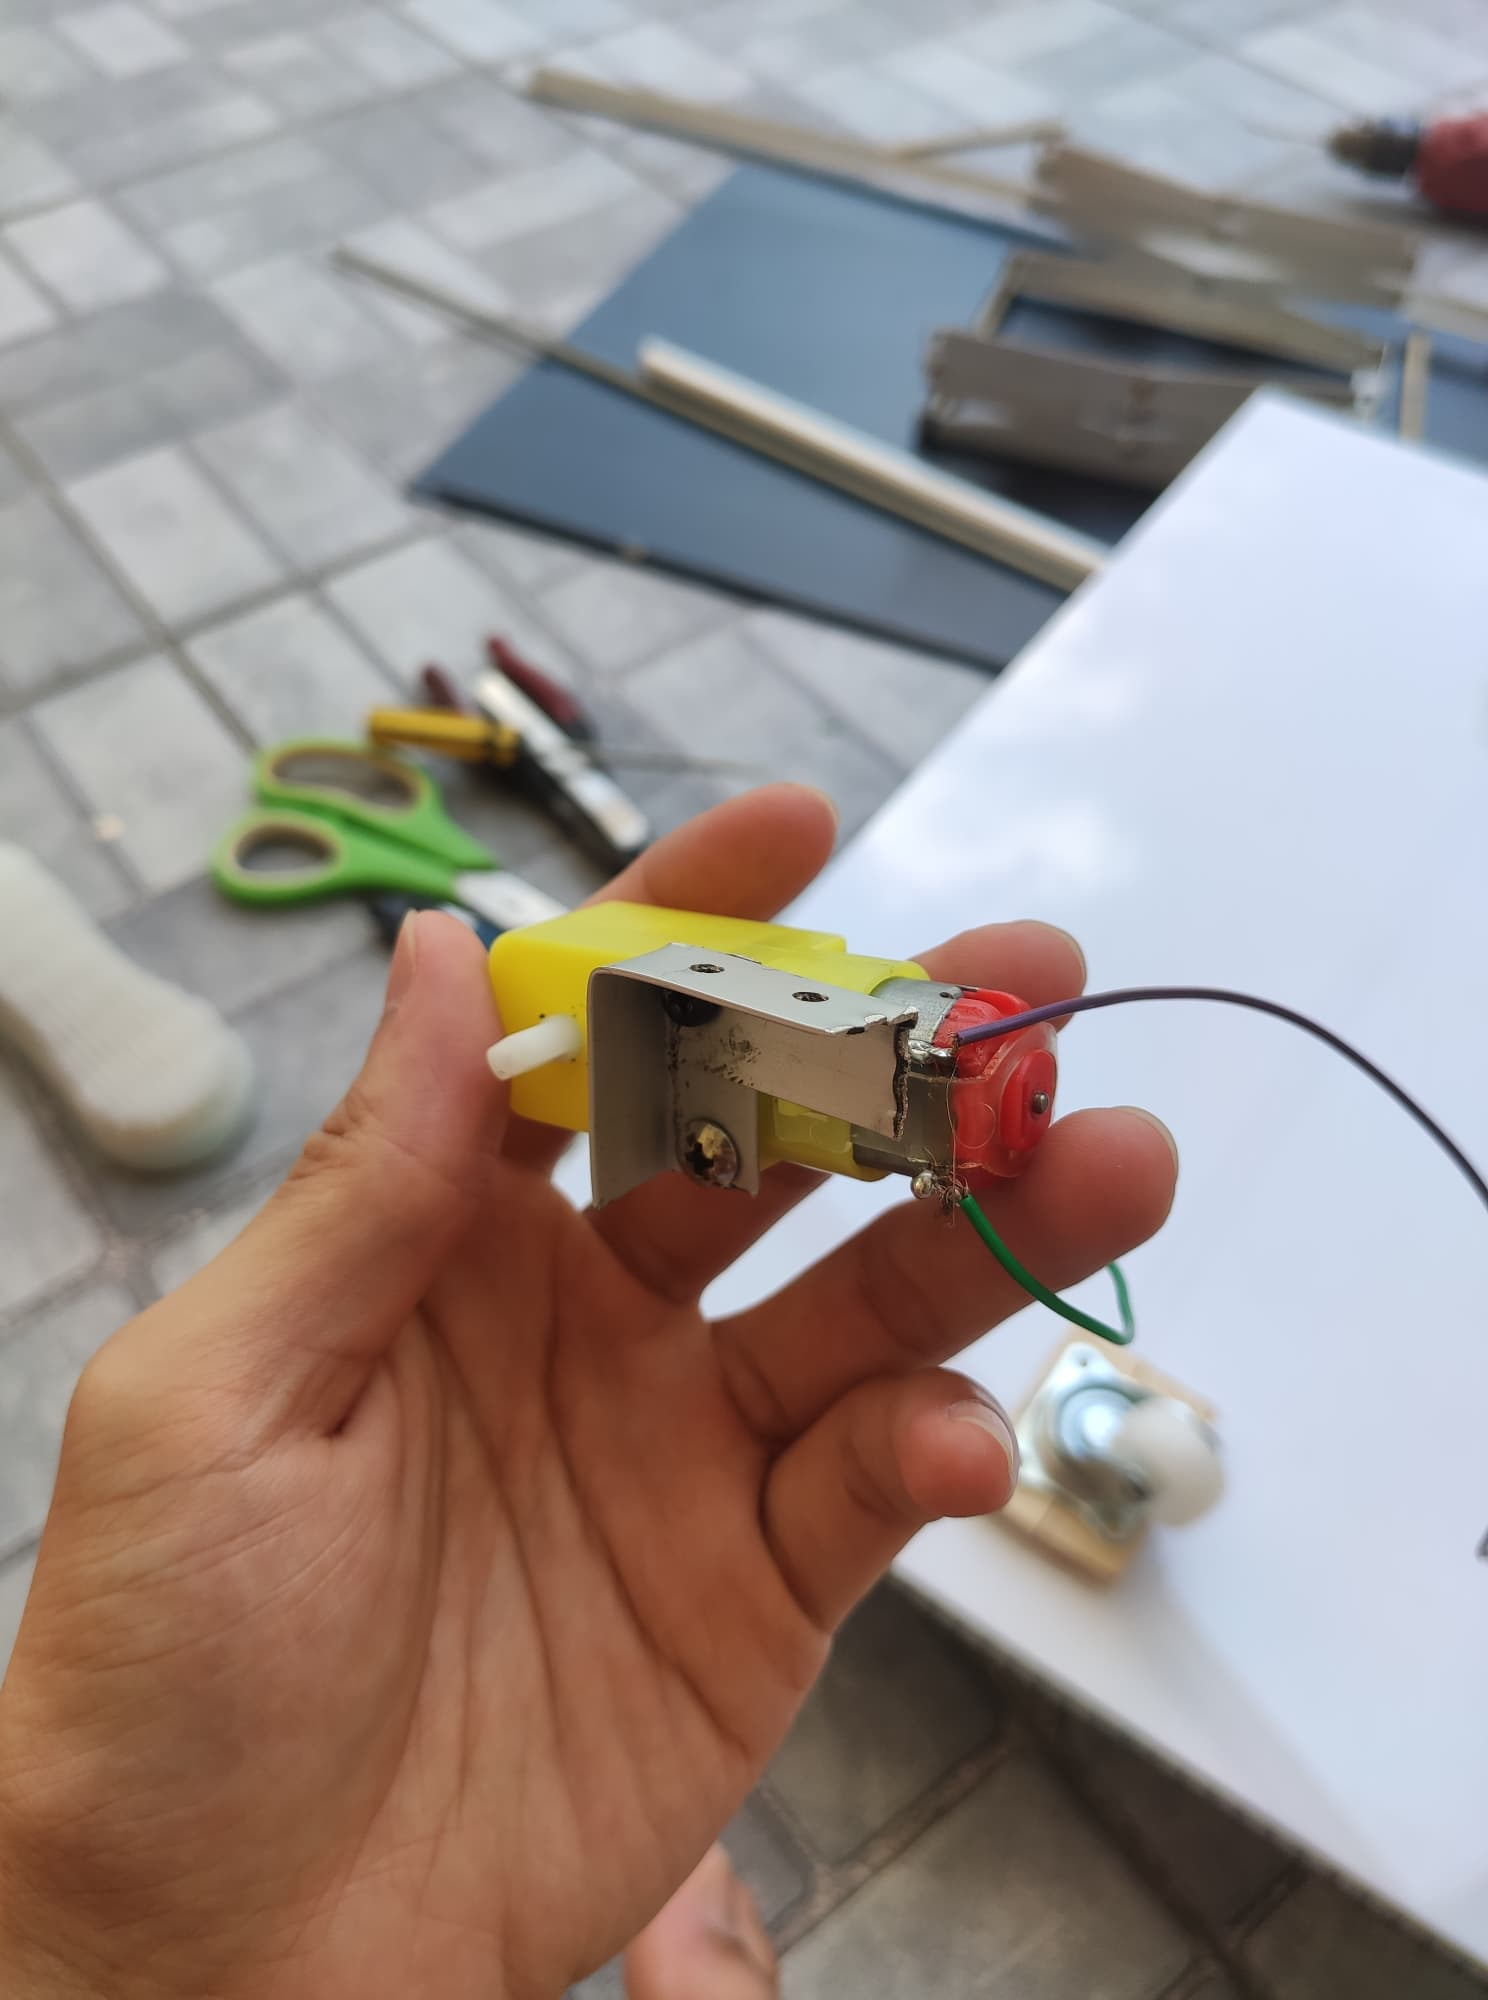
\includegraphics[height= 5cm]{M4}}
	\caption{Reinforcing equipment} \label{fig:m3m4}
\end{figure}

\par 

Forthly, a model of scissor lift was created then a scissor lift was built and attached to the body of the trolley.

\begin{figure}[H]
	\centering
	\subfloat[Model of a scissor lift \label{fig:m5}]{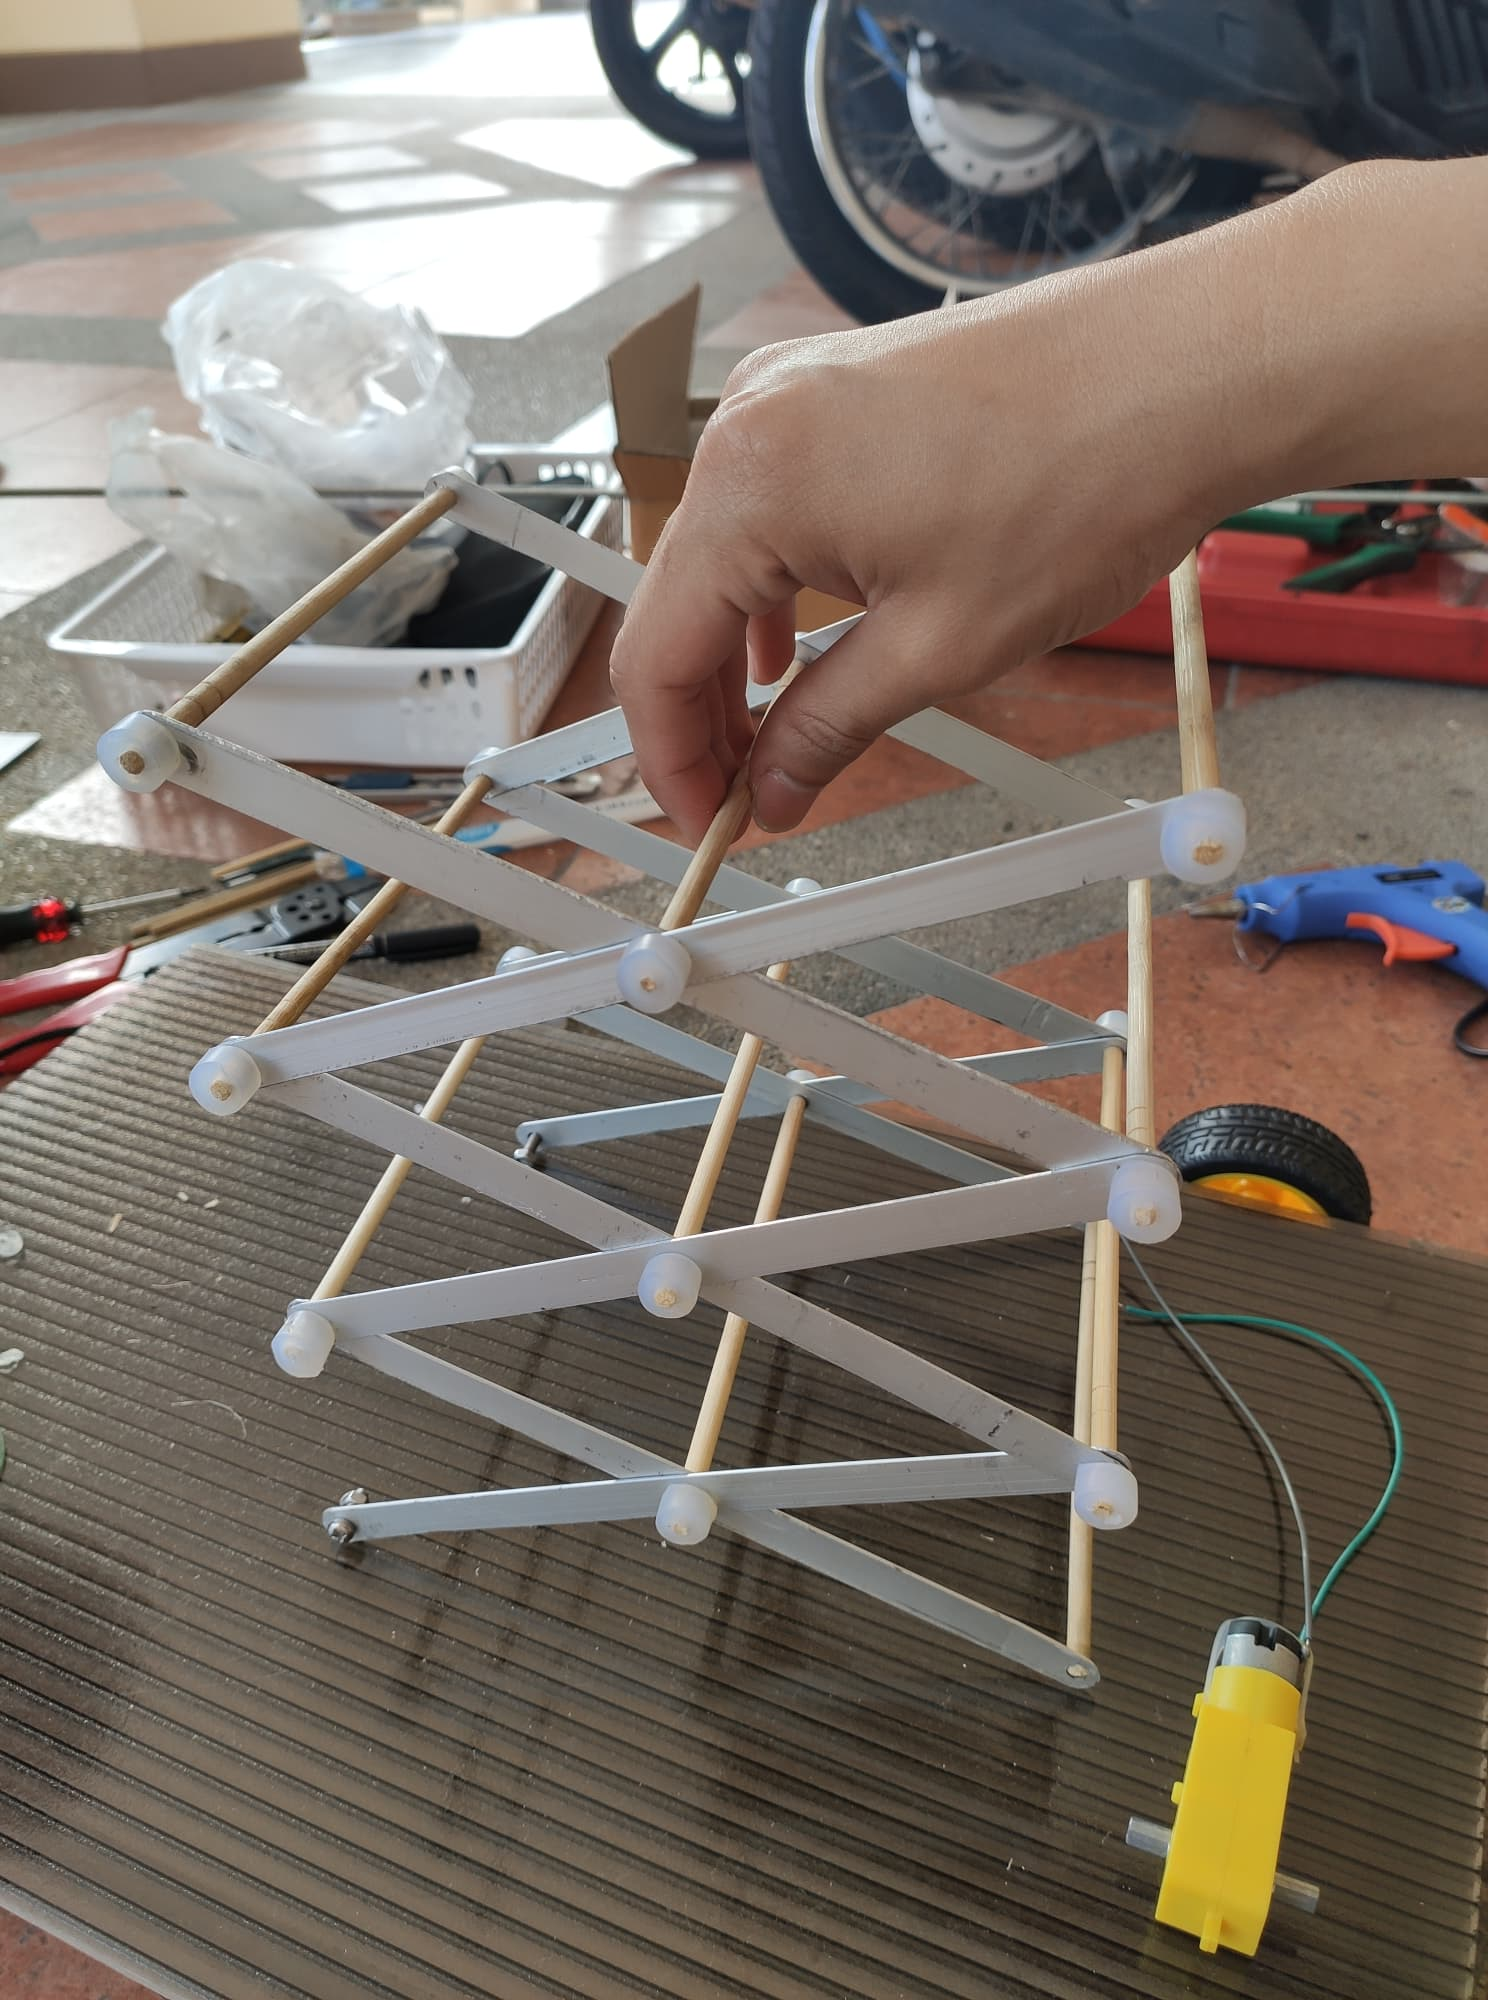
\includegraphics[height= 5cm]{M5}} \hspace{1cm}
	\subfloat[Scissor lift \label{fig:m6}]{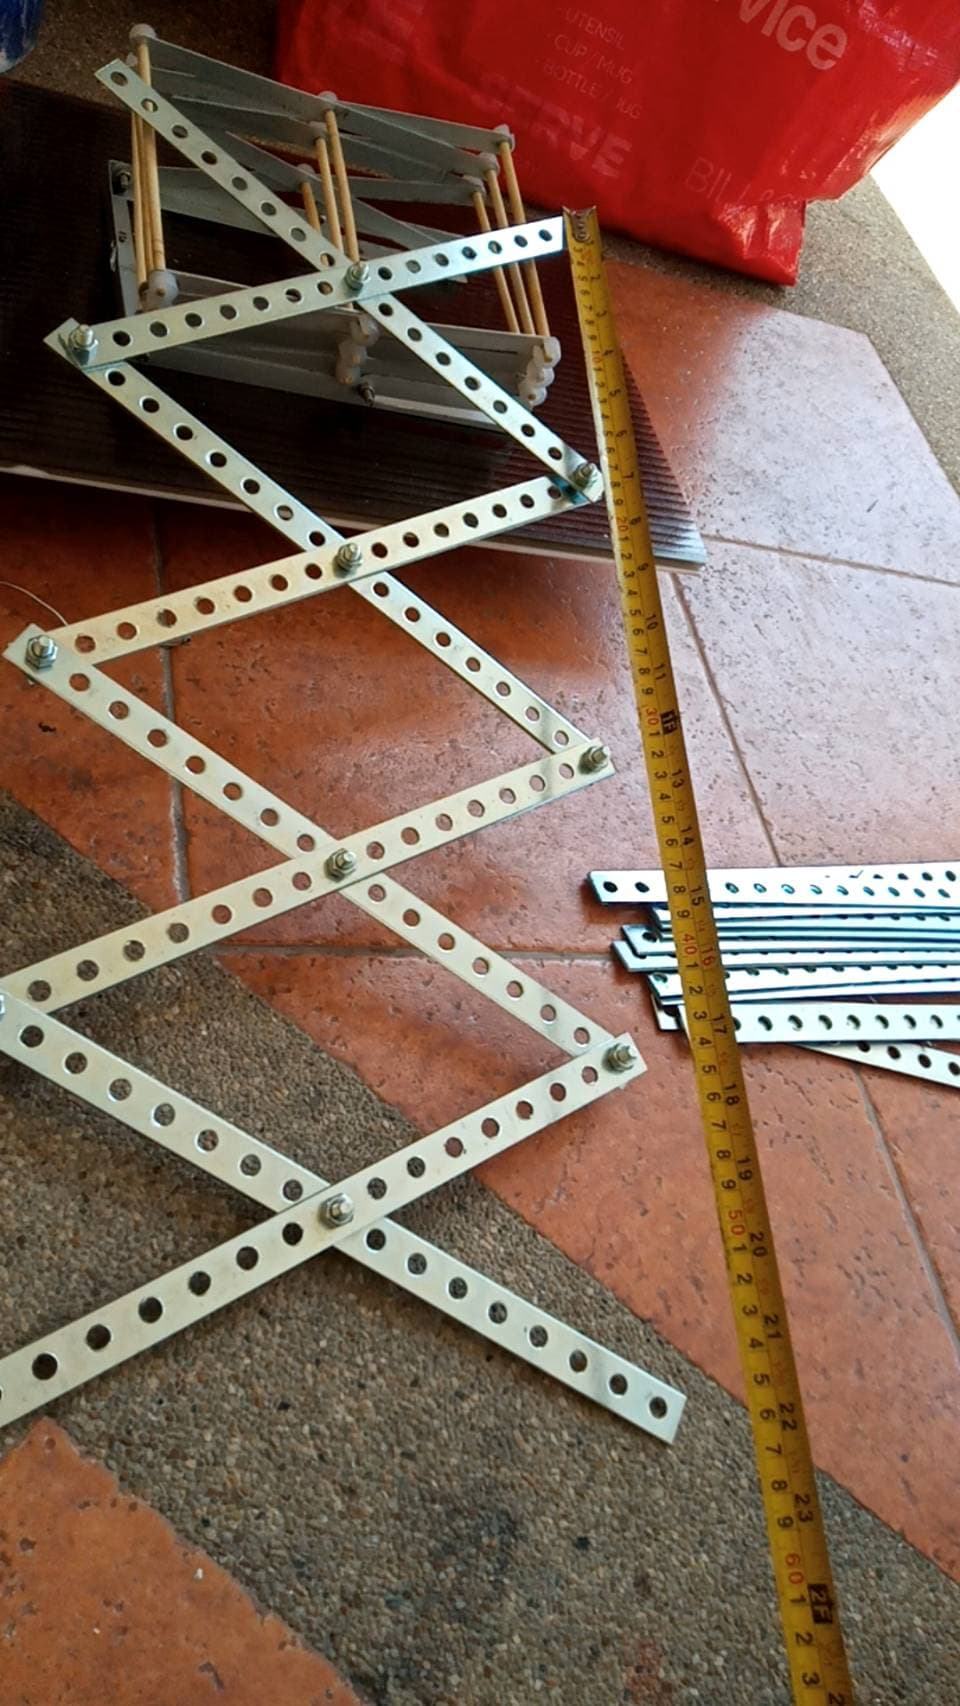
\includegraphics[height= 5cm]{M6}} \\ \vspace{0.5cm}
	\subfloat[Scissor lift \label{fig:m7}]{\includegraphics[height= 4cm]{m7}}
	\caption{Model of a scissor lift and a scissor lift} \label{fig:m3m4}
\end{figure}

% \section{Experiment and Result} \label{sec:experiment} %

\section{Conclusion} \label{sec:conclusion}

\subsection{Work done} \label{subsec:workdone}

The goal of our project is to make a delivery system that can deliver small object such as paperwork and to demonstrate how easy of automation is.\par
Currently, we have completely built our DIY trolley and tested our system. The DIY trolley can run smoothly to the station and to the parking lot, the trolley can wirelessly connect to the phone application and the phone application can communicate with the trolley.

\subsection{Future work} \label{subsec:futurework}

There are many options that the trolley can be improved and developed. The camera can be attach to the trolley to provide vision to the sender and receiver. Moreover, the LIDAR (Light Detection and Ranging) can be used instead of the ultra sonic sensor since LIDAR provide better function for avoiding obstacle. 

\nocite{*}
\bibliographystyle{ieeetr}
\bibliography{References}
\addcontentsline{toc}{section}{\numberline{}References}

\newpage

\appendix
\section{Coding} \label{sec:coding}
\subsection{Motors and Ultrasonic Code} \label{sub:}
\texttt{\lstinputlisting{MotorUltrasonicCode.ino}}





\end{document}
